\documentclass[a4paper]{master}



%Information as title and author
\title{Simulation of Jet D'Eau from A to Y:\\ Numerical algorithm to solve incompressible Navier-Stokes equations
with \textcolor{blue}{m}arker \textcolor{blue}{a}nd \textcolor{blue}{c}ell based method}
\author{Pablo Strasser}
\Supervisor{Prof. Martin Gander and Dr. Felix Kwok}
\date{\today}

%Pdf information
\hypersetup{pdfinfo={%
  Title={Master Thesis},
  Author={Pablo Strasser},
  Creator={Pablo Strasser},
  Producer={Pablo Strasser},
  Subject={Navier-Stockes},
  Keywords={Navier-Stockes}}
}

\tikzexternalize

\begin{document}
\captionsetup{singlelinecheck=off,margin=10pt,font=small,labelfont=bf}
%make the title page
\maketitle
\dominitoc

\chapter*{Abstract}

\mtcaddchapter[Abstract]

We will in this work present how to solve Navier-Stokes equations with a marker and cell method.
We use direct Navier-Stokes approach without other model than the Navier-Stokes equations.
We emphasy the mathematical modularity which allow to work separatly on every piece of this work.
Our method work for every Runge-Kutta method (explicit or implicit), if we note $k$ the order of the choosen Runge-Kutta method,
our method is of order $k$ if we ignore boundary conditions, of order $k$ at the better case and of order $1$ for specific complicated case.
Our method is exactly divergence free (at numerical precision).

We will specially be interested in free surface boundary conditions. The final goal is to solve a Jet d'Eau.
This goal was only partially achieved, but the needed basics are there. 


\tableofcontents

\chapter*{Introduction}

\mtcaddchapter[Introduction]

This work consists of the following chapters:
\begin{enumerate}
 \item A notation and basic math property chapter.
 \item A chapter that describe the problem analytically. In this chapter no discretization is done, but equations are written in the good form to motivate discretization.
 \item A chapter that is interested on the solution of Navier-Stokes equations if the domain of computation is fixed.
 \item A chapter that indicate the change needed to allow domain change.
 \item To end, a conclusion chapter which will contain pist to upgrade the scheme used.
\end{enumerate}

The two numerical chapters contain pseudo code that implement the described algorithm.

The original \textbf{C++11} code can be found on \url{https://github.com/Strasser-Pablo/Mac}
but is not needed to understand this work, the pseudo code is sufficient.

All the chapters are self contained,
but further information and inspiration come from:
\begin{itemize}
 \item Algorithmic idea like the layer variable and the first scheme come from \cite{fluidforrestofus}.
 \item Analytical comprehension and better formulation come from \cite{citeulike:11163809}.
 \item Extrapolation for boundary conditions come from \cite{FLD:FLD148}.
 \item Analytical solution are taken from \cite{Batchelor} and \cite{Kampanis:2006:SGH:1148052.1148065}.
 \item A review of marker and cell based method can be found in \cite{citeulike:3055787}.
\end{itemize}



\chapter{Introduction}

\section{Introduction}

\section{Notation and Somes Basic Math Property}

\subsection{Vector}

Vector with the dimension of physical space (2d or 3d) are written $\vect{v}$.

We only use cartesian coordinate system.

We indicate a given component of a vector with indice. $\vect{v}_1$ is the first component.

\subsection{Differential operator}

\subsubsection{Component by component}

Derivatif is written $\partial_i$ where $i$ is the spatial component with witch we derivate.
\begin{equation}
 \partial_i v(\vect{x})=\frac{\partial v(\vect{x})}{\partial \vect{x}_{i}}
\end{equation}

\subsubsection{Nabla}

\begin{definition}
 In Cartesian coordinate, the $\vect{\nabla}$ is a vector that cannot commute.
 It's expression is given by:
 \begin{equation}
 \vect{\nabla}_{i}=\partial_{i}
 \end{equation}
\end{definition}

With the $\vect{\nabla}$ we can form the following expression.
With $n$ the dimension of the vector:
\begin{equation}
 \vect{\nabla}p=\begin{pmatrix}\partial_1 p\\ \vdots \\ \partial_n p\end{pmatrix}
\end{equation}
\begin{equation}
 \vect{\nabla}\cdot \vect{v}=\sum_{i=1}^{n}\partial_i \vect{v}_i
\end{equation}
\begin{equation}
 \left((\vect{v}\cdot\vect{\nabla})\vect{v}\right)_{i}=\sum_{j=1}^{n}v_{j}\partial_{j} v_{i}
\end{equation}

\subsubsection{Laplacian}

\begin{definition}
The lapplacian $\Delta$ consist of a scalar operator witch can be seen as:
\begin{equation}
\Delta=\vect{\nabla}\cdot \vect{\nabla}=\sum_{i=1}^{n} \partial_{i}\partial_{i}
\end{equation}
\end{definition}

\begin{definition}
A vector version of the laplacian consist to apply the laplacian to all component of the vector.
We note the vector version of the laplacian $\vect{\Delta}$
\end{definition}
\subsection{Divergence Free and Rotational Free Space}

\subsubsection{Definition}

\begin{definition}
 The Divergence of a vector consist of:
 \begin{equation}
  \vect{\nabla} \cdot \vect{v}
  \end{equation}
\end{definition}

\begin{definition}
 The Rotational of a vector consist of:
 \begin{equation}
  \vect{\nabla} \times \vect{v}
 \end{equation}
\end{definition}

\begin{definition}
 The Gradiant of a scalar consist of:
 \begin{equation}
  \vect{\nabla} p
 \end{equation}
\end{definition}

\subsubsection{Property}

\begin{property}
 The divergence of a vector is Rotational Free.
 \begin{equation}
  \vect{\nabla}\times \vect{\nabla} p=\vect{0}
 \end{equation}
\end{property}

\begin{property}
 The gradiant of a vector is Divergence Free.
 \begin{equation}
  \vect{\nabla}\cdot \vect{\nabla} \vect{v}=0
 \end{equation}
\end{property}
\subsubsection{Projection}

\label{introduction:projection}
\begin{property}
 Every vector can be projected to a divergence free space without changing it's rotational with the following change:
\begin{align}
 \vect{v_{new}}&=v-\vect{\nabla}p \label{introduction:ProjectionA}\\
 \Delta p&=\vect{\nabla} \cdot \vect{v} \label{introduction:ProjectionB}
\end{align}
\end{property}
\begin{proof}
  Taking the divergence of equation \ref{introduction:ProjectionA} and using \ref{introduction:ProjectionB}
  \begin{equation}
   \vect{v_{new}}=\vect{\nabla}\cdot\vect{v}-\Delta p=\vect{\nabla}\cdot\vect{v}-\vect{\nabla}\cdot\vect{v}=0
  \end{equation}
  \begin{rem}
 This work as long as:
 \begin{equation}
  \Delta=\vect{\nabla}\cdot \vect{\nabla}\label{introduction:ProjectionDelta}
 \end{equation}
 So this can be used in discretized case and will be exact as long as \ref{introduction:ProjectionDelta} is respected.
 \end{rem}
\end{proof}


\chapter{Analytical problem and analytical result}

\minitoc
\section*{Introduction}
In this chapter, we will discuss the analytical problem that we want to solve.
The other numerical chapters will consist of numericals schemes to solve the problem given in this chapter.

\section{Variables and parameters}

The problem will consist to find a function of space and time in a certain domain respecting some conditions and equations.

We begin to define space, time and domain:
\begin{description}
\item[The \emph{space}] consists of a vector in fixed Cartesian coordinate with dimension typically 2 or 3 (Navier-Stokes on 1d is trivial).
Space is noted $\vect{x}$.
\item[The \emph{time}] consists of a indice indicating the evolution of the function in time.
Time is noted $t$.
\item[The \emph{domain}] is the spatial region where a field is defined. This consists physically in the spatial region where water lies.
Boundary conditions need to be provided.
The domain can vary with respect of time and can vary with respect of the solution at previous time.
The domain doesn't need to be connected. But can be decomposed in union of connected subdomain.

\begin{example}
 If we take a drop of water falling in a glass of water. The domain consist of the region where the water lies.
 At the beginning this will consist of domain consisting of two connected subdomains (the drop and the glass)
 that after a given time will merge in one domain.
\end{example}

The domain is generally noted $\Omega$ or $\Omega(t)$ to emphasize that it can be variable with respect of time.
\end{description}

The variable of the equation are named \emph{Field} and consists of functions with respect of space in the spatial domain and time in the temporal domain.
\begin{equation}
 F(x,t)\qquad \text{With $x\in\Omega(t)$ and $t_0\leq t \leq t_f$}
\end{equation}

We have the following fields:
\begin{description}
\item[The \emph{speed}:] A vector field consisting of the speed in space and time.
The speed is noted $\vect{v}$.
\item[The \emph{pressure}:] A scalar field consisting of an internal force per unit area in the fluid.
We will not use the pressure in this work, but the pressure divided by density.
If we note the pressure $\tilde{p}$ we use:
\begin{equation}
 p=\frac{\tilde{p}}{\rho}
\end{equation}
Because we use incompressible Navier-Stokes equation, $\rho$ is constant. This can be view as a change of unit.
\end{description}

The following constant parameters are used:
\begin{description}
\item[The \emph{viscosity}] represents how much water particles stick together.
Higher is the viscosity less abrupt speed changes are possible.
The viscosity is noted $\mu$. We use allot $\nu$ that is the viscosity divided by the density.
\begin{equation}
 \nu=\frac{\mu}{\rho}
\end{equation}
\item[The \emph{density}] is a mass per unit volume.
Density play the same role as mass in Newton's mechanic.
In the incompressible Navier-Stokes equation density is a constant because incompressibility tells us that density doesn't change.
The density is noted $\rho$.
\item[The \emph{external force}] is a user defined vector field that represents the external force applied to the water.
It can possibly depends on the solution for previous time.
The force is noted $\vect{F}$.
\end{description}

\section{Navier-Stokes equations}

\subsection{Fixed eulerian topology}
\label{analytical:fixe_eulerian}
The incompressible Navier-Stokes equations are given by:
\begin{subequations}
\begin{align}
\label{analytical:navierStokesA}
\vect{\nabla} \cdot \vect{v}(\vect{x} ,t)&=0\\
\label{analytical:navierStokesB}
\partial_t \vect{v}(\vect{x} ,t)+(\vect{v}(\vect{x},t)\cdot\vect{\nabla} ) \vect{v}(\vect{x} ,t)&=-\vect{\nabla} p(\vect{x},t)+\frac{\vect{F}(\vect{x},t)}{\rho(\vect{x},t)}+\nu \Delta \vect{u}(\vect{x},t)
\end{align}
\end{subequations}

Equation \ref{analytical:navierStokesA}, tells us that the speed is a divergence free field.
Equation \ref{analytical:navierStokesB} is an equation of evolution. The presence of $p$ allows to maintain the speed always divergence free.
Taking the rotational of \ref{analytical:navierStokesB} make disappear the pressure term (because the rotational of a gradient is 0).

The pressure term can be seen as a correction of the divergence without changing the rotational.

We can rewrite Navier-Stokes equations as:
\begin{subequations}
\begin{align}
\label{analytical:navierStokesRewA}
\vect{\nabla} \cdot \vect{v}(\vect{x} ,t)&=0\\
\label{analytical:navierStokesRewB}
\partial_t \vect{v}(\vect{x} ,t)&=f(\vect{v}(\vect{x},t))-\vect{\nabla}p
\intertext{Where}
f(\vect{v}(\vect{x},t))&=-(\vect{v}(\vect{x},t)\cdot\vect{\nabla} ) \vect{v}(\vect{x} ,t)+\frac{\vect{F}(\vect{x},t)}{\rho(\vect{x},t)}+\nu \Delta \vect{u}(\vect{x},t)
\end{align}
\end{subequations}

Taking the divergence of equation \ref{analytical:navierStokesRewB} we found:
\begin{equation}
  \Delta p=\vect{\nabla}\cdot f(\vect{v})
\end{equation}
But using the notation of \ref{introduction:projectiondef}:
\begin{equation}
	-\vect{\nabla}p=P(f(\vect{v}))
\end{equation}

The equations of Navier-Stokes are then equivalent to solve:
\begin{equation}
  \partial_t \vect{v}(\vect{x} ,t)=f(\vect{v}(\vect{x},t))+P(f(\vect{v}(\vect{x},t))=(\eye+P)f(\vect{v}(\vect{x},t))
\end{equation}
$(\eye+P)$ is a projector on a divergence free space without changing the rotational.

\subsection{Mobile eulerian topology }
When topology is variable, we need to add another equation to tell where is the domain of computation.
A natural boundary condition is the free surface, wich moves with the speed at given point.

We define $\lambda$ a system of representative. And $\vect{\xi}_{\lambda}$ the position of point given by $\lambda$.
The domain is given by the union of $\vect{\xi}$ for all $\lambda$.

The Navier-Stokes equations are now:
\begin{subequations}
\begin{align}
\label{analytical:navierStokesMobA}
\vect{\nabla} \cdot \vect{v}(\vect{x} ,t)&=0\\
\label{analytical:navierStokesMobB}
\partial_t \vect{v}(\vect{x} ,t)+(\vect{v}(\vect{x},t)\cdot\vect{\nabla} ) \vect{v}(\vect{x} ,t)&=-\vect{\nabla} p(\vect{x},t)+\frac{\vect{F}(\vect{x},t)}{\rho(\vect{x},t)}+\nu \vect{\Delta} \vect{u}(\vect{x},t)\\
\partial_t \vect{\xi}_{\lambda}(t)&=\vect{v}(\vect{\xi}_{\lambda},t)
\end{align}
\end{subequations}
We can as in section \ref{analytical:fixe_eulerian} eliminate the constrain on the divergence with the same notation:
\begin{subequations}
\begin{align}
\partial_t \vect{v}(\vect{x} ,t)&=f(\vect{v}(\vect{x},t))+P(f(\vect{v}(\vect{x},t))=(\eye+P)f(\vect{v}(\vect{x},t))\\
\partial_t \vect{\xi}_{\lambda}(t)&=\vect{v}(\vect{\xi}_{\lambda},t)\label{ana:move:equ}
\end{align}
\end{subequations}

\subsection{Lagrangian form of Navier-Stokes equations}
\label{analytical:convectif}
We will in this section rewrite \ref{analytical:navierStokesB} in another form.
We begin to define a new position system (which is similar to the particle position used in previous section) $\vect{\xi}_{\lambda}(t)$:
\begin{subequations}
\begin{align}
 \partial_t \vect{\xi}_{\lambda}(t)&=\vect{v}(\vect{\xi}_{\lambda}(t),t)\\
 \vect{\xi}_{\lambda}(t_0)&=\vect{\xi}^{0}_{\lambda}
\end{align}
\end{subequations}
$\lambda$ is a system of representative that is initialized by initial condition.
For a given $\lambda$, $\vect{\xi}_{\lambda}(t)$ follows the speed at the given point.
This position system is called particle coordinate or Lagrangian.
$\vect{\xi}_\lambda(t)$ is called the characteristic.

We then can define the Lagrangian speed.
\begin{equation}
 \vect{u}_{\lambda}(t)=\vect{v}(\vect{\xi}_{\lambda}(t),t)
\end{equation}
The Lagrangian speed is the speed following a characteristic.

Taking the total derivative (the derivative of everything that depend on time) of the Lagrangian speed with respect of time, we have:
\begin{equation}
\frac{d \vect{u}_{\lambda}(t)}{d t}=\frac{d \vect{v}(\xi_{\lambda},t)}{d t}=\partial_t \vect{v}+\left(\frac{\partial \vect{\xi}_{\lambda}(t)}{\partial t}\cdot\vect{\nabla}\right)\vect{v}
\end{equation}
This can be rewritten:
\begin{equation}
\frac{d \vect{u}_{\lambda}(t)}{d t}=\partial_t \vect{v}+\left(\vect{v} \cdot\vect{\nabla}\right)\vect{v}
\end{equation}
This is exactly the lhs of equation \ref{analytical:navierStokesB}.

We then can rewrite Navier-Stokes equations as:
\begin{subequations}
\begin{align}
\label{analytical:navierStokesLagA}
\vect{\nabla} \cdot \vect{u}_{\lambda}(t)&=0\\
\label{analytical:navierStokesLagB}
\frac{d \vect{u}_{\lambda}(t)}{d t}&=-\vect{\nabla} p(\vect{\xi}_{\lambda}(t),t)+\frac{\vect{F}(\vect{\xi}_{\lambda}(t),t)}{\rho(\vect{x},t)}+\nu \Delta \vect{u}_{\lambda}(t)
\end{align}
\end{subequations}

\begin{remark}
We remark that with this notation some expression like spatial derivative of $\vect{u}$ is not defined.
In an analytical procedure, we can transform $\vect{u}$ to $\vect{v}$ with the help of the expression of $\vect{\xi}$, then the derivative is well defined.
But in a numerical procedure, the point where the values are know are particles. This demand to define derivative on unstructured grid
or to interpolate at grid point.
\end{remark}

\section{Boundary conditions}

We will be interested in two kinds of boundary conditions.
\begin{description}
 \item[\emph{Inflow} Boundary:]
 An inflow boundary is a source of water.
 \item[\emph{free surface} Boundary:]
 A free surface boundary is a freely moving boundary where the other fluid is inert.
\end{description}

\subsection{Inflow}

Inflow boundary conditions have a constant prescribed speed.
This give the following constraint on pressure:
\begin{equation}
\nabla p(\vect{x},t)=f(\vect{v}(\vect{x},t))
\end{equation}

The following alternative boundary conditions have been used.
Set the speed on the surface artificially to constant and use 0 Neumann boundary conditions.


\subsection{Free surface}
\label{ana:free:surface}
To define the free surface boundary conditions, we need to define the stress tensor:
\begin{equation}
	\sigma_{ij}=-p \delta_{ij}+\nu\left(\frac{\partial v_{i}}{\partial x_{j}}+\frac{\partial v_{j}}{\partial x_{i}}\right)
\end{equation}
The boundary conditions are then given by (for 3d):
\begin{align}
	\sum_{i,j}\sigma_{ij}n_{i}n_{j}&=0\\
	\sum_{i,j}\sigma_{ij}t^{1}_{i}n_{j}&=0\\
	\sum_{i,j}\sigma_{ij}t^{2}_{i}n_{j}&=0\\
\end{align}
Where $\vect{n}$ is the normal vector and $\vect{t}^1$ and $\vect{t}^2$ are two non-colinear tangent vectors.
For 2d only one tangent vector is needed.

The first equation can be used to find boundary conditions for $p$.
The other equations only depend of speed, because $\vect{n}$ is orthogonal to $\vect{t}^{1}$ and $\vect{t}^{2}$.
The value of $\nu$ is not relevant for the condition (a global non zero constant).
The constraint is linear.
\chapter{Fixed}
\minitoc
\section{Introduction}

We will in this chapter be interested in the case of fixed domain Navier-Stokes with grid discretisation.
This case is easier than the variable domain case and serve as basis to more complicated case.

\section{Overview}

To solve the Navier-Stokes equation, we will cut the equation in two step.
\begin{enumerate}
\item Evolve speed without consideration of pressure and divergence free.
  \begin{equation}
  \partial_t \vect{v}(\vect{x} ,t)+(\vect{v}(\vect{x},t)\cdot\vect{\nabla} ) \vect{v}(\vect{x} ,t)=\frac{\vect{F}(\vect{x},t)}{\rho(\vect{x},t)}+\nu \Delta \vect{u}(\vect{x},t)
  \end{equation}
\item We project the none divergence free speed found before to a divergence free speed.
  \begin{align}
  \vect{v}_{new}&=v-\vect{\nabla}\phi\\
  \Delta \phi&=\vect{\nabla} \cdot \vect{v}
  \end{align}
\end{enumerate}

After this step the discrete evaluation of divergence will be divergence free exactly (to numerical precision) as long as the shame used respect:
\begin{equation}
\Delta=\vect{\nabla}\cdot \vect{\nabla}
\end{equation}

\begin{rem}
This method to have a divergence free speed is different that what we will find if we use the analytical expression for $p$ found in equation \ref{analytical:pressure}:
\begin{equation}
  \Delta p=-\rho \vect{\nabla} \cdot (\vect{v}\cdot \vect{\nabla}) \vect{v}
\end{equation}

But using this equation, will not ensure in the numerical case that the speed is divergence free.
The latter equation will not be used because we consider that being divergence free at every time step is more important than
to have the good equation for pressure but where time discretisation error will create more divergence.
\end{rem}

\section{Evolve in time}

We need to solve:
  \begin{equation}
  \partial_t \vect{v}(\vect{x} ,t)=\frac{\vect{F}(\vect{x},t)}{\rho(\vect{x},t)}+\nu \Delta \vect{u}(\vect{x},t)-(\vect{v}(\vect{x},t)\cdot\vect{\nabla} ) \vect{v}(\vect{x} ,t)
  \end{equation}
  
  \subsection{Analytical solution to Burger's equation}
  This equation is know as the Burger equation and can be solved analytically for $\nu=0$.
  The solution is given by the method of characteristics. Using the same method that we us in section \ref{analytical:convectif}.
  \begin{equation}
  \frac{d u_{\lambda}(t)}{dt}=\frac{\vect{F}(\vect{x},t)}{\rho(\vect{x},t)}
  \end{equation}
  
  The change of speed is given by the force.
  
  This equation can after a finite time have more that one solution and don't have continuous and derivable solution everywhere.
  
  We see this in taking for example a sinus as input speed for the case without force.
  The high speed region of the sinus will go faster than the slow point of the sinus.
  After a given time we will find a multi-valued solution. This is the sign, that we need to consider discontinuous solution after this time.
  But solution are no more unique, other condition need to be added.
  
  For the 3d case of Navier-Stokes equation we do not know if we have unicity after a given time.
  We know that we have a solution but not how many.
  
  In discretized version, we only need to solve for one time step.
  The projection step will change the speed everywhere.

  \subsection{Method of Line}
  
  A typical method of resolution is to discretize in time and space separately.
  We consider that the Burger equation is given by:
  \begin{align}
  \label{fixed:lineA}
  \partial_t \vect{v}(\vect{x} ,t)&=f(\vect{v}(\vect{x}),\vect{x})\\
  \label{fixed:lineB}
  f(t,\vect{v}(\vect{x}),\vect{x})&=\frac{\vect{F}(\vect{x},t)}{\rho(\vect{x},t)}+\nu \Delta \vect{u}(\vect{x},t)
  \end{align}
  
Equation \ref{fixed:lineA} is now an ordinary differential equation for a field $\vect{v}$.
Equation \ref{fixed:lineB} is the evaluation of an expression with derivative at a given time and position.

\subsubsection{Runge-Kutta}

A Runge-Kutta method is a method to solve the ODE (I drop the $\vect{x}$ dependence, but it's understood that this equation is for a vector formed in concatenating every speed):
\begin{equation}
\partial_t \vect{v}(t)=f(\vect{v})
\end{equation}

The solution at time $n+1$ is given from the solution at time $n$ with $\Delta t$ the time step and $a$, $b$ parameter of the method.
\begin{align*}
	\vect{v}_{n+1}&=\vect{v}_{n}+\sum_{i=1}^{s}b_{i}k_{i}\\
	k_{j}&=\Delta t f(\vect{v}_{n}+\sum_{i=1}^{j-1}a_{j,i}k_{i})
\end{align*}

\subsubsection{Spatial Evaluation}
To apply the Method of Line, we need to evaluate derivative.

\section{Projection}
\label{fixed:projection}
The projection step consist to apply:
\begin{align}
  \vect{v}_{new}&=v-\vect{\nabla}\phi\\
  \Delta \phi&=\vect{\nabla} \cdot \vect{v}\label{fixed:project}
\end{align}

Equation \ref{fixed:project} typically consist to solve a linear system.

\section{Runge-Kutta and Projection}

A possible idea, is to project after every evaluation of speed int the Runge-Kutta method.
We first define the projection for a vector $\vect{v}$, $P(\vect{v})$.
Using \ref{fixed:projection} $P(\vect{v})$ can be written:
\begin{equation}
  P(\vect{v})=-\vect{\nabla}\left(\vect{\nabla}\cdot \vect{\nabla}\right)^{-1}\vect{\nabla}\cdot\vect{v}
\end{equation}

$P$ is a linear operator because derivative are linear operator.

From the Navier-Stokes equation:
\begin{equation}
  \partial_t \vect{v}(\vect{x} ,t)=-(\vect{v}(\vect{x},t)\cdot\vect{\nabla} ) \vect{v}(\vect{x} ,t)+\frac{\vect{F}(\vect{x},t)}{\rho(\vect{x},t)}+\nu \Delta \vect{u}(\vect{x},t)-\nabla \phi
\end{equation}

Can be rewritten:
\begin{align}
\label{fixed:rung-projA}
  \partial_t \vect{v}(\vect{x} ,t)&=f(\vect{v})-\nabla \phi \\
  \intertext{With:}
  f(\vect{v})&=-(\vect{v}(\vect{x},t)\cdot\vect{\nabla} ) \vect{v}(\vect{x} ,t)+\frac{\vect{F}(\vect{x},t)}{\rho(\vect{x},t)}+\nu \Delta \vect{u}(\vect{x},t)
\end{align}

Taking the divergence of \ref{fixed:rung-projA} we can determine $\phi$.
\begin{equation}
  \Delta \phi=\nabla \cdot f(\vect{v})
\end{equation}

The gradient of $\phi$ is then:

\begin{equation}
  -\vect{\nabla}\phi=P(f(\vect{v}))
\end{equation}

The Navier-Stokes equation can then be rewritten as:
\begin{equation}\label{fixed:simpl_navier}
\partial_t \vect{v}(\vect{x} ,t)=f(\vect{v})+P(f(\vect{v})) 
\end{equation}

This equation is analytically exact.

We would expect that solving this equation with a Runge-Kutta algorithm will lead to a numerical error in Divergence.

To show that this is not the case, we show that another method to force divergence free of every speed is in fact equivalent to this one.

We define the following scheme.
\begin{align}
\vect{\tilde{v}}_{n+1}&=\vect{\tilde{v}}_{n}+\sum_{i=1}^{s}b_{i}\tilde{k}_{i}+P\left(\vect{\tilde{v}}_{n}+\sum_{i=1}^{s}b_{i}\tilde{k}_{i}\right)\\
\tilde{k}_{i}&=\Delta t f\left(\vect{\tilde{v}}_{n}+\sum_{j=1}^{i-1}a_{ij}\tilde{k}_{j}+P\left(\vect{\tilde{v}}_{n}+\sum_{j=1}^{i-1}a_{ij}\tilde{k}_{j}\right)\right)
\end{align}

We project at every estimation of speed. Making by construction every speed divergence free.

We now write the Runge-Kutta expression for \ref{fixed:simpl_navier}.

\begin{align}
	\vect{v}_{n+1}&=\vect{v}_{n}+\sum_{i=1}^{s}b_{i}k_{i}\\
	k_{i}&=\Delta t f\left(\vect{v}_{n}+\sum_{j=1}^{i-1}a_{ij}k_{j}\right)+\Delta t P\left(f\left(\vect{v}_{n}+\sum_{j=1}^{i-1}a_{ij}k_{j}\right)\right)
\end{align}

\begin{thm}
If $\vect{v}_{n}=\vect{\tilde{v}}_{n}$ and $\vect{v}_n$ is divergence free then $\vect{v}_{n+1}=\vect{\tilde{v}}_{n+1}$ 
\end{thm}
\begin{proof}
We begin by prove the following lemma.
\begin{lem}
\begin{equation}
  k_{i}=\tilde{k}_{i}+P(\tilde{k}_{i})
\end{equation}
\end{lem}
\begin{proof}
By recurrence on $i$.
We begin with $i=1$:
\begin{equation}
  k_{1}=\Delta tf\left(\vect{v}_n\right)+\Delta tP\left(f\left(\vect{v}_n\right)\right)
\end{equation}
\begin{equation}
\tilde{k}_{1}=\Delta tf\left(\vect{v}_n\right)
\end{equation}
\begin{equation}
  k_{1}=\Delta t f\left(\vect{v}_n\right)+\Delta tP\left(f\left(\vect{v}_n\right)\right)=\tilde{k}_1+P\left(\tilde{k}_1\right)
\end{equation}

Assuming true for smaller $i$:
\begin{align*}
  k_{i}&=\Delta tf\left(\vect{v}_n+\sum_{j=1}^{n}a_{ij}k_{j}\right)+\Delta tP\left(f\left(\vect{v}_n+\sum_{j=1}^{i-1}a_{ij}k_{ij}\right)\right)\\
  &=\Delta tf\left(\vect{v}_n+\sum_{j=1}^{i-1}a_{ij}\left(\tilde{k}_{j}+P\left(\tilde{k}_{j}\right)\right)\right)+\Delta tP\left(f\left(\vect{v}_n+\sum_{j=1}^{i-1}a_{ij}\left(\tilde{k}_{j}+P\left(\tilde{k}_{j}\right)\right)\right)\right)\\
  \tilde{k}_{i}&=\Delta tf\left(\vect{v}_n+\sum_{j=1}^{i-1}a_{ij}\tilde{k}_{j}+P\left(\vect{v}_n+\sum_{j=1}^{i-1}a_{ij}\tilde{k}_{j}\right)\right)\\
  &=\Delta tf\left(\vect{v}_n+\sum_{j=1}^{i-1}a_{ij}\left(\tilde{k}_{j}+P\left(\tilde{k}_{j}\right)\right)\right)\\
  k_{i}&=\tilde{k}_{i}+P\left(\tilde{k}_{i}\right)
\end{align*}
\end{proof}

We now write the expression for $\vect{v}_{n+1}$ and $\vect{\tilde{v}}_{n+1}$ using the lemma.

\begin{align*}
\vect{v}_{n+1}&=\vect{v}_{n}+\sum_{i=1}^{s}b_{i}k_{i}\\
&=\vect{v}_{n}+\sum_{i=1}^{s}b_{i}\left(\tilde{k}_{i}+P\left(\tilde{k}_{i}\right)\right)\\
\vect{\tilde{v}}_{n+1}&=\vect{\tilde{v}}_{n}+\sum_{i=1}^{s}b_{i}\tilde{k}_{i}+P\left(\vect{\tilde{v}}_{n}+\sum_{i=1}^{s}b_{i}\tilde{k}_{i}\right)\\
&=\vect{\tilde{v}}_{n}+\sum_{i=1}^{s}b_{i}\left(\tilde{k}_{i}+P\left(\tilde{k}_{i}\right)\right)\\
\intertext{Using that $\vect{v}_{n}=\tilde{\vect{v}_{n}}$}
\vect{v}_{n+1}&=\vect{\tilde{v}}_{n+1}
\end{align*}

\end{proof}

\begin{thm}
For the implicit Runge-Kutta case, where the sum to $i-i$ go now to $s$.
If $\vect{v}_{n}=\vect{\tilde{v}}_{n}$ and $\vect{v}_n$ is divergence free then $\vect{v}_{n+1}=\vect{\tilde{v}}_{n+1}$ 
\end{thm}
\begin{proof}
We begin by prove the following lemma.
\begin{lem}
\begin{equation}
  k_{i}=\tilde{k}_{i}+P(\tilde{k}_{i})
\end{equation}
\end{lem}
\begin{proof}
Because the sum goes to $s$ and not $i-1$ we cannot use recurrence.
We now will use vector notation for $k$.

We construct $k$ and $\tilde{k}$ vector with the vector $k_{i}$ and $\tilde{k}_{i}$
\begin{align}
k&=\begin{pmatrix}
    k_{1}\\
    \vdots\\
    k_{s}\\
  \end{pmatrix}\\
\tilde{k}&=\begin{pmatrix}
    \tilde{k}_{1}\\
    \vdots\\
    \tilde{k}_{s}\\
  \end{pmatrix}
\end{align}

We form $\hat{P}$ and $\hat{f}$ from a Kronecker product:
\begin{align}
\hat{P}&=\eye_{s}\kron P=\begin{pmatrix}P	&\ldots	&0\\
			\vdots &\ddots 	&\vdots\\
			0	&0	&P\\
	\end{pmatrix}\\
\hat{f}&=\eye_{s}\kron f\begin{pmatrix}f	&\ldots	&0\\
			\vdots &\ddots 	&\vdots\\
			0	&0	&f\\
	\end{pmatrix}
\end{align}

We now define $\hat{v}_n$:
\begin{equation}
\hat{v}_{n}=\begin{pmatrix}
	      v_{n}\\
	      \vdots\\
	      v_{n}
	      \end{pmatrix}
\end{equation}

We now define $A$ with the following Kronecker product:
\begin{equation}
A=\begin{pmatrix}
    a_{11}	&\ldots	&a_{1s}\\
    \vdots	&\ddots	&\vdots\\
    a_{s1}	&\ldots	&a_{ss}\\
  \end{pmatrix} \kron \eye
\end{equation}

$A$ and $\hat{P}$ are commutative, because of the mixed-product property.
\begin{align}
A\hat{P}&=\left(\begin{pmatrix}
    a_{11}	&\ldots	&a_{1s}\\
    \vdots	&\ddots	&\vdots\\
    a_{s1}	&\ldots	&a_{ss}\\
  \end{pmatrix} \kron \eye \right)
  \left(\eye_{s}\kron P\right)=
	\begin{pmatrix}
    a_{11}	&\ldots	&a_{1s}\\
    \vdots	&\ddots	&\vdots\\
    a_{s1}	&\ldots	&a_{ss}\\
    \end{pmatrix}\kron P\\
    %
    \hat{P}A&=
  \left(\eye_{s}\kron P\right)
	\left(\begin{pmatrix}
    a_{11}	&\ldots	&a_{1s}\\
    \vdots	&\ddots	&\vdots\\
    a_{s1}	&\ldots	&a_{ss}\\
  \end{pmatrix} \kron \eye \right)=
	\begin{pmatrix}
    a_{11}	&\ldots	&a_{1s}\\
    \vdots	&\ddots	&\vdots\\
    a_{s1}	&\ldots	&a_{ss}\\
    \end{pmatrix}\kron P
\end{align}

\begin{align}
k&=(1+\hat{P})\Delta t\hat{f}(\hat{v}_{n}+Ak)\\
\tilde{k}&=\Delta t \hat{f}((1+\hat{P})(\hat{v}_{n}+Ak))
\end{align}

We begin to define 2 functions:
\begin{align}
k&=g(k)\\
\tilde{k}&=\tilde{g}(\tilde{k})\\
g(x)&=(1+\hat{P})\Delta t \hat{f}(\hat{v}_{n}+Ax)\\
\tilde{g}(x)&=\Delta t \hat{f}((1+\hat{P})(\hat{v}_{n}+Ax))
\end{align}

$k$ and $\tilde{k}$ are fixed point of function $g$ and $\tilde{g}$.

We now calculate:
\begin{align}
(1+\hat{P})\tilde{g}(x)&=(1+\hat{P})\Delta t \hat{f}((1+\hat{P})(\hat{v}_{n}+Ax))=(1+\hat{P})\Delta t \hat{f}(\hat{v}_{n}+A (1+\hat{P})x)\\
&=g((1+\hat{P})x)
\end{align}

We now substitute $g$ in $\tilde{g}$
\begin{equation}
(1+\hat{P})\tilde{k}=g((1+\hat{P})\tilde{k})
\end{equation}

$(1+\hat{P})\tilde{k}$ is a fixed point of $g$.
But fixed point of $g$ is $k$.

\begin{equation}
k=(1+\hat{P})\tilde{k}
\end{equation}
This is exactly the vector version of what we wanted to prove.
\end{proof}

The rest is exactly the same than in the first case:

We now write the expression for $\vect{v}_{n+1}$ and $\vect{\tilde{v}}_{n+1}$ using the lemma.

\begin{align*}
\vect{v}_{n+1}&=\vect{v}_{n}+\sum_{i=1}^{s}b_{i}k_{i}\\
&=\vect{v}_{n}+\sum_{i=1}^{s}b_{i}\left(\tilde{k}_{i}+P\left(\tilde{k}_{i}\right)\right)\\
\vect{\tilde{v}}_{n+1}&=\vect{\tilde{v}}_{n}+\sum_{i=1}^{s}b_{i}\tilde{k}_{i}+P\left(\vect{\tilde{v}}_{n}+\sum_{i=1}^{s}b_{i}\tilde{k}_{i}\right)\\
&=\vect{\tilde{v}}_{n}+\sum_{i=1}^{s}b_{i}\left(\tilde{k}_{i}+P\left(\tilde{k}_{i}\right)\right)\\
\intertext{Using that $\vect{v}_{n}=\tilde{\vect{v}_{n}}$}
\vect{v}_{n+1}&=\vect{\tilde{v}}_{n+1}
\end{align*}

\end{proof}

\begin{cor}
Solving Navier-Stokes equation with the analytical good choice of pressure.
Is exactly divergence free at every approximation of speed.
\end{cor}
\begin{proof}
  The expression of $v$ is the solution of the Navier-Stokes equation with the good choice of pressure.
  $\tilde{v}$ is the solution of Runge-Kutta equation without pressure witch is projected at every speed estimation.
  This is divergence free.
  $v$ and $\tilde{v}$ are the same. With end the proof.
\end{proof}

\begin{cor}
  Using the expression for $v$ or $\tilde{v}$ we are $k$ order precise in time. Where $k$ is the order of the Runge-Kutta method.
\end{cor}
\begin{proof}
  $v$ and $\tilde{v}$ are the same.
  $v$ consist only of a Runge-Kutta method with a good chosen function.
  So the order in time of $v$ and $\tilde{v}$ is the same that the method order.
\end{proof}


\chapter{Numerical treatment of the non fixed case }
\minitoc
\section{Introduction}
In the previous chapter all numerical schemes were done on the same domain.
We will see here the changes that we need to make if we want to have a variable topology.
We will need to take care of two additional things:
\begin{enumerate}
\item Knowing the speed in cell that were not in the domain but are in the new time step.
\item Knowing the position of the different boundary.
\end{enumerate}

We are mainly interested in a mobile boundary consisting of a free surface boundary because it will be the only
boundary that moves depending on the solution.

The motion of the domain and the boundary are given by:
\begin{equation}
\dot{\vect{x}}=\vect{v},
\end{equation}
where $\vect{v}$ is the speed at the given position.

The spatial space is discretized into a set of cells. Cells coincide with cells in the staggered grid discretization.
The domain is a union of cells.
To discretize this equation, we will use particles  placed in every cell. A cell where a particle lies is in the domain.
A cell without particle is outside of the domain.
But particles move with the speed given at their position, which is not on a grid point.
Because of this, we need to interpolate the speed at the given point.
When a particle moves to a new cell, we need to know the initial speed at this position.
We analytically have boundary conditions for speed at boundary.
We need to extrapolate this boundary condition one cell away.

\section{Method to obtain an ODE}

We can write a non discretized particle method equation as:
\begin{align*}
	\dot{v}&=\left(\eye - P(D(\vect{x}))\right)f(\vect{v},\vect{x}),\\
	\dot{x}&=v,\\
	x&=x_{0},
\end{align*}
Where $x$ is a continuous representation of the space with particle.
$D(\vect{x})$ is the domain with particle in it.
The notation $P(D(\vect{x}))$ says that we consider the projection operator with boundary conditions in the domain given by $D(\vect{x})$.

We need to add to this boundary conditions, boundary conditions for free surface, that are given by a linear differential operator $A$,
\begin{equation}
	A\vect{v}=0.
\end{equation}
$A$ contains derivatives with respect to space but not with respect to time.

When we discretize, we will need to interpolate because we need the speed at position not on the grid (for a staggered grid we have):
\begin{align*}
	\left.\dot{\vect{v}}\right|_{\in D_{v}(D(\vect{x}))}&=\left(\eye+P(D(\vect{x}))\right)\left.f(E(\vect{v},D_v(D(\vect{x}))),D_{v}(D(\vect{x})))\right|_{\in D_{v}(D(\vect{x}))},\\
	\dot{x}&=I\left(\vect{x},E(\vect{v},D_v(D(\vect{x})))\right),\\
	\left.\vect{v}\right|_{\notin D_{v}(D(\vect{x}))}&=\left.E(\vect{v},D_v(D(\vect{x})))\right|_{\notin D_{v}(D(\vect{x}))}.
\end{align*}
For mathematical simplicity we will assume that $\vect{v}$ consists of a speed defined everywhere, 
but in the computation only the speeds that are accessed in the time step are needed (only the speed in the domain and in its neighbour).
We can model this by considering non used cells with a special value like NaN that propagates in every operation.
\begin{description}
\item[$D(\vect{x})$] indicates the domain in which at least one particle is found. This corresponds at the same time to the topology for pressure (Pressure is cell centered).
\item[$D_{v}$] is a function depending on the topology given in general by $D(\vect{x})$ and indicates which speed components are in the domain.
\item[$f$] is a function that takes as argument the topology for pressure given by $D(\vect{x})$ and the topology for speed given by $D_v(D(\vect{x}))$ and the speed everywhere.
\item[$E$] extends the velocity field defined in the domain to the total spatial space.
This is implemented by a extrapolation operator which takes as argument the speed everywhere and returns a speed everywhere,
but where the speed in the speed domain is not changed. This speed is the speed that the fluid had if it were there.
The distance to which this extrapolation operator needs to give values depends on the choice of the time step.
The extrapolation operator needs to take into account two things:
\begin{enumerate}
	\item The correct boundary conditions.
	\item Extrapolate speed farther away than the boundary conditions if a particle moves more than one cell.
\end{enumerate}
\item[$I$] is an interpolation operator which from the speed at discrete position finds the speed at a given position.
\end{description}
The use of two topologies is needed because on a staggered grid the position of speed and pressure is not the same.

\begin{remark}
$D_{v}$ needs to be well chosen to avoid pathological cases.
For example for a domain with only one cell. We will normally consider all speed as boundary. But with only boundary we have no speed data.
For this reason in this case, we consider all boundary cell as being in the domain.
\end{remark}


\subsection{Splitting}
\label{splitting}

A simple, but only of order $1$ (in general) method to solve these equations, is to consider two different problems:
\begin{enumerate}
	\item Advance speed for a given topology.
	\item Advance the particle from the given speed.
\end{enumerate}
The first step is to solve:
\begin{align}
\left.\dot{\vect{v}}\right|_{\in D_{v}(D(\vect{x}))}&=\left(\eye+P(D(\vect{x}))\right)\left.f(E(\vect{v},D_v(D(\vect{x}))),D_{v}(D(\vect{x})))\right|_{\in D_{v}(D(\vect{x}))},\\
	\left.\vect{v_{t_0}}\right|_{\notin D_{v_{t_0}}(D(\vect{x}))}&=\left.E(\vect{v_{t_0}},D_v(D(\vect{x})))\right|_{\notin D_{v}(D(\vect{x}))},
\end{align}
which can be done like in the fixed topology case with a Runge-Kutta method. The second equation indicates the boundary conditions.
Numerically we can calculate the speed at the boundary at every evaluation of $f$.

We then move the particles with the calculated speed,
\begin{equation}
	\dot{x}=I\left(\vect{x},E(\vect{v},D_v(D(\vect{x})))\right).\\
\end{equation}
This method is only of order 1.

\begin{example}
Consider only one particle. With as initial condition $0$ speed without viscosity.

The extrapolation operator in this case will copy the speed vertically,
the speed will be constant and the only non zero component is in the $y$ direction.
The speed will be given by the integration of the gravity force, the convective term is $0$ because speed is constant.
The speed will be calculated with an accuracy of the order of the Runge-Kutta method used (4 for rk4).
The exact solution for speed (which is constant in space) is:
\begin{equation}
 v_y(t)=-gt^2.
\end{equation}
But the position will be calculated from the advance of a constant speed for every time step. This is then equivalent to the Euler
method of order 1.

In conclusion, our speed will be correct to order $k$ for a given time step but the position will be inacurate.

This error doesn't depend on the precision of integration for the speed or position problem.
It comes from the splitting.
\end{example}

\subsection{One ODE method}
\label{differentialequation}
We will now show how we can rewrite this differential equation in only one differential equation.
For this, we need an expression for the derivative of the boundary condition.
When we have it, we only have to use a Runge-Kutta method.


We will now only be interested in the case where $E$ is a linear operator with the two following constraints:
\begin{itemize}
	\item Its effect for speed in the domain (for speed) is the identity.
	\item Its effect for speed outside of the domain (for speed) depends only on the speed of the domain (for speed).
\end{itemize}
The domain for speed for $E$ is denoted by $E(D_v(D(\vect{x})))$.

In matrix notation it tells us that some blocks need to be $0$ or $\eye$.
If we consider that indices from $1$ to $n_d$ are in the domain (for speed) and $n_d+1$ to $n$ are outside of the domain (for speed), the constraint for a line of the matrix is,
using as notation the : as in matlab in indicating by an indice its position in the vector:
\begin{align}
	\intertext{For $i<n_d+1$}
	E_{i :}&=\left( 0 \ldots 1_{i} \ldots 0\right)\\
	\intertext{For $i>n_d$}
	E_{i :}&=\left( e^i_{1}\ldots e^i_{n_d} 0\ldots 0\right)\\
\end{align}

Taking the derivative of $E(D_v(D(\vect{x})))\vect{v}$ has two terms, the first gives:
\begin{equation}
	E(D_v(D(\vect{x})))\dot{\vect{v}},
\end{equation}
which uses $\dot{\vect{v}}$ but needs it only for the domain because outside the given column of the $E$ matrix is zero.

The second term is the derivative of the matrix $E$ with respect to change of time, which will lead to the derivative with respect to the change of topology.
This will give a delta of Dirac.
The reason of this is because of the discontinuity in time of the boundary speed, when we change topology.
We will neglect this Dirac delta. Neglecting this Dirac delta is a dangerous steps but the problem is not as big at it could seem at first.
It will be explained in details after.

The equation is then:
\begin{align}
	\left.\dot{\vect{v}}\right|_{\in D_{v}(D(\vect{x}))}&=\left(\eye+P(D(\vect{x}))\right)\left.f(E(D_v(D(\vect{x})))\vect{v},D_{v}(D(\vect{x})))\right|_{\in D_{v}(D(\vect{x}))},\\
	\left.\dot{\vect{v}}\right|_{\notin D_{v}(D(\vect{x}))}&=E(D_v(D(\vect{x})))\left(\eye+P(D(\vect{x}))\right)\left.f(E(D_v(D(\vect{x})))\vect{v},D_{v}(D(\vect{x})))\right|_{\in D_{v}(D(\vect{x}))},\\
	\left.\vect{v_{t_0}}\right|_{\notin D_{v_{t_0}}(D(\vect{x}))}&=\left.\left(E(D_v(D(\vect{x})))\left.\vect{v_{t_0}}\right|_{\in D_{v}(D(\vect{x}))}\right)\right|_{\notin D_{v}(D(\vect{x}))},\\
	\dot{x}&=I\left(\vect{x},E(D_v(D(\vect{x})))\vect{v}\right),\\
\end{align}
where we have used the notation that vector can be extended with 0 when needed because the extension is not needed because the good columns are zero,
which can be rewritten as:
\begin{align}\label{topo:equ:onediff}
	\dot{\vect{v}}&=E(D_v(D(\vect{x})))\left(\eye+P(D(\vect{x}))\right)\left.f(E(D_v(D(\vect{x})))\vect{v},D_{v}(D(\vect{x})))\right|_{\in D_{v}(D(\vect{x}))},\\
	\left.\vect{v_{t_0}}\right|_{\notin D_{v_{t_0}}(D(\vect{x}))}&=\left.\left(E(D_v(D(\vect{x})))\left.\vect{v_{t_0}}\right|_{\in D_{v}(D(\vect{x}))}\right)\right|_{\notin D_{v}(D(\vect{x}))},\\
	\dot{x}&=I\left(\vect{x},E(D_v(D(\vect{x})))\vect{v}\right),\\
\end{align}
where we have used that $E$ is the identity in the domain.
This equation can be integrated with a Runge-Kutta method.
For maximal precision, the boundary speed is taken from the extrapolation at every complete Runge-Kutta step.
In the argument of $f$ we have used an extrapolation of speed which does not depend on the input in boundary speed (because the $E$ matrix has zero columns where needed).
The integrated boundary speed is only used in the case where a cell becomes a domain cell in a time step.

The neglected Dirac delta will only have an effect on a boundary speed component in the case where in a Runge-Kutta step the following happens:
\begin{enumerate}
	\item A neighboring cell (cell which $E$ matrix has component with) fills.
	This will change the value of boundary speed with a jump (this jump will be neglected).
	\item The given speed is used because a particle fills the domain.
	This is needed because in the contrary the speed calculated will not be used.
\end{enumerate}
This effect is shown in figure \ref{topo:mult_part_error}.
This effect will change the precision when it happens from order $k$ to order $1$.
And this error will only be on the boundary conditions being not exactly respected for a short time.
The force will be integrated correctly.

The direct filling of a cell does not pose a problem because we do not have a discontinuity in speed, because in the first region we force speed,
in the second the derivative.
The jump is only caused because we force speed differently for the two regions which give a discontinuity.

\begin{example}
One particle with 0 initial speed, without viscosity.
The speed will be constant. So only the gravity force acts and the extrapolation operator will copy speed vertically.
The result will then be equivalent to the integration of the pure particle problem where the speed change is calculated at particle position.
The order of the method is then $k$.
The calculation of this example is done in section \ref{top:exp:one}.
\end{example}

\tikzsetnextfilename{multiple_part_error_1}
 \tikzifexternalizing{\directlua{dofile('topology/multiple_part_error_1.lua')}}{
 \IfFileExists{figures/multiple_part_error_1.pdf}{}{
\begin{tikzpicture}
\end{tikzpicture}}
}
 \tikzsetnextfilename{multiple_part_error_2}
 \tikzifexternalizing{
\directlua{dofile('topology/multiple_part_error_2.lua')}
}{
\IfFileExists{figures/multiple_part_error_2.pdf}{}{
\begin{tikzpicture}
\end{tikzpicture}
}
}
  \tikzsetnextfilename{multiple_part_error_3}
 \tikzifexternalizing{
\directlua{dofile('topology/multiple_part_error_3.lua')}
}{
\IfFileExists{figures/multiple_part_error_3.pdf}{}{
\begin{tikzpicture}
\end{tikzpicture}
}
}
\begin{figure}
\centering
\subcaptionbox{$t_0$, the red speed vector is not in the domain and is obtained by extrapolation.\label{topo:mult_part_error:1}}{%
\IfFileExists{figures/multiple_part_error_1.pdf}{\includegraphics{figures/multiple_part_error_1}}{}%
 }
\subcaptionbox{$t_1$, because the first particle has moved the domain haves changed, the speed extrapolation haves changed at the red point.\label{topo:mult_part_error:2}}{%
\IfFileExists{figures/multiple_part_error_2.pdf}{\includegraphics{figures/multiple_part_error_2}}{}%
 }
\subcaptionbox{$t_2$, because the red point is now in the domain, the speed is given by the acceleration from the Navier-Stokes equations.\label{topo:mult_part_error:3}}{%
\IfFileExists{figures/multiple_part_error_3.pdf}{\includegraphics{figures/multiple_part_error_3}}{}%
 }
\subcaptionbox{Cartoon of speed, the topology at time $t_0$, $t_1$ and $t_2$
are given in \ref{topo:mult_part_error:1} , \ref{topo:mult_part_error:2} and \ref{topo:mult_part_error:3}.
$t_{in}$ is the moment when particle $1$ enters in the new cell.$t_{f}$ is the moment when particle $2$ enters in the new cell.
The red curve is what we will integrate if we neglect the delta of Dirac, the black curve is the exact result.\label{topo:mult_part_error:4}}{
\tikzset{external/export next=false}
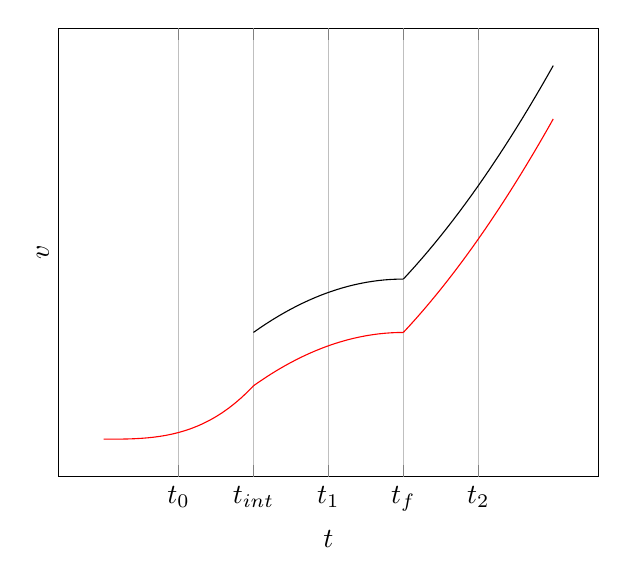
\begin{tikzpicture}
  \begin{axis}[xtick=\empty,ytick=\empty, extra x ticks={0.5,1,1.5,2,2.5},
extra x tick style={grid=major},
extra x tick labels={$t_0$,$t_{int}$,$t_1$,$t_{f}$,$t_2$ },
xlabel={$t$},
ylabel={$v$}
]
   \addplot[domain=0:1,red] {x^3};
   \addplot[domain=1:2] {-(x-2)^2+3};
   \addplot[domain=1:2,red] {-(x-2)^2+2};
   \addplot[domain=2:3,red] {3*x-4+(x-2)^2};
   \addplot[domain=2:3] {3*x-3+(x-2)^2};
  \end{axis}

 \end{tikzpicture}
}
\caption{Figure of the situation where the neglected delta has a effect.}
\label{topo:mult_part_error}
\end{figure}


\section{Extrapolation}

We will now discuss how to define the extrapolation operator.
We have seen that the extrapolation operator needs to do two things:
\begin{enumerate}
	\item Ensure correct boundary conditions.
	\item Extrapolate the rest of speed.
\end{enumerate}

We now are interested in enforcing the boundary condition.
Numerically this will be done by extrapolating the value at exterior from the boundary conditions on the derivative.
One important point is how we enforce the boundary conditions on the discrete grid.
We recall our equation of section \ref{ana:free:surface}:
\begin{align}
	\sum_{i,j}\sigma_{ij}n_{i}n_{j}&=0,\\
	\sum_{i,j}\sigma_{ij}t^{1}_{i}n_{j}&=0,\\
	\sum_{i,j}\sigma_{ij}t^{2}_{i}n_{j}&=0.\\
\end{align}
Because the constraints are linear, with sufficiently additional equation (divergence free) and know value we can find an unique solution.

We now will treat the different possible cases in 2d. This will then be generalized to 3d.
We will use different discretisation points for pressure and speed.
We begin with the discretisation for speed.

\subsection{2d}
\label{topo:extrap:2d}
\subsubsection{Plane}

The first case is a surface which is a plane following one of the cell boundaries.
Without loss of generality we consider the plane in the $x$ direction (the other case are just rotations of this case).
The normal and tangent vectors are then given by:
\begin{align}
	\vect{n}&=\begin{pmatrix}
			0\\
			1
		\end{pmatrix},\\
	\vect{t}&=\begin{pmatrix}
			1\\
			0
		\end{pmatrix}.
\end{align}
The equation is then given by:
\begin{align}
	\sum_{i,j}\sigma_{ij}t_{i}n_{j}&=0,\\
	\sigma_{12}&=0\\
	-p \delta_{12}+\nu\left(\frac{\partial v_{1}}{\partial x_{2}}+\frac{\partial v_{2}}{\partial x_{1}}\right)&=0,\\
	\frac{\partial v_{1}}{\partial x_{2}}+\frac{\partial v_{2}}{\partial x_{1}}&=0.\\
\end{align}

We discretize this equation at point $i+\frac{1}{2},j+\frac{1}{2}$:
\begin{equation}
\label{var:extr:droitCont}
	\frac{v^{1}_{i+\frac{1}{2},j+1}-v^{1}_{i+\frac{1}{2},j}}{\Delta x_{2}}+\frac{v^{2}_{i+1,j+\frac{1}{2}}-v^{2}_{i,j+\frac{1}{2}}}{\Delta x_{1}}=0,
\end{equation}
where $\Delta x_{1}$ and $\Delta x_{2}$ are the spacings in $x$ and $y$.
We have one equation for 3 unknowns, only $v^{1}_{i+\frac{1}{2},j}$ are known.
But we can add two equations using the divergence free condition in the fluid for cell $i,j$ and $i+1,j$.
This gives us:
\begin{align}
\label{var:extr:droitContA}
	0&=\frac{v^{1}_{i+\frac{1}{2},j}-v^{1}_{i-\frac{1}{2}},j}{\Delta x_{1}}+\frac{v^{2}_{i,j+\frac{1}{2}}-v^{2}_{i,j-\frac{1}{2}}}{\Delta x_2},\\
\label{var:extr:droitContB}
	v^{2}_{i,j+\frac{1}{2}}&=v^{2}_{i,j-\frac{1}{2}}-\frac{v^{1}_{i+\frac{1}{2},j}-v^{1}_{i-\frac{1}{2},j}}{\Delta x_{1}}\Delta x_{2},\\
\label{var:extr:droitContC}
	0&=\frac{v^{1}_{i+\frac{3}{2},j}-v^{1}_{i+\frac{1}{2}},j}{\Delta x_{1}}+\frac{v^{2}_{i+1,j+\frac{1}{2}}-v^{2}_{i,j-\frac{1}{2}}}{\Delta x_2},\\
\label{var:extr:droitContD}
	v^{2}_{i+1,j+\frac{1}{2}}&=v^{2}_{i+1,j-\frac{1}{2}}-\frac{v^{1}_{i+\frac{3}{2},j}-v^{1}_{i+\frac{1}{2},j}}{\Delta x_{1}}\Delta x_{2}.
\end{align}
We substitute the two equations (\ref{var:extr:droitContB}) and (\ref{var:extr:droitContD}) in equation (\ref{var:extr:droitCont}),
which will now only depend on one unknown $v^{1}_{i+\frac{1}{2},j+1}$ which depends on a quantity that can be found using the speed in the domain.
Figure \ref{topology:extrap:plane} shows the variables used and the unknowns.

We can do the things that we have done only if we have a depth of minimal two cells.
If we have only one cell, we have no $y$ speed in the domain of calculation.
For this case, consider the speed $y$ at the boundary as in the domain and let it evolve without constraint.

\begin{figure}
\directlua{dofile('topology/plane_extrapolation.lua')}
\caption{The red point is the place where the boundary condition is discretized.
The green dots are cells where the divergence free rule is enforced. Red vectors are calculated with respect to the blue one.}
\label{topology:extrap:plane}
\end{figure}

\subsubsection{\unit{45}{\degree} plane}

If we have a cell in the domain with two adjacent cells which are not in the domain,
we take as normal a \unit{45}{\degree} plane.

The normal and tangent vectors are then:
\begin{align}
	\vect{n}&=\begin{pmatrix}
	\frac{\sqrt{2}}{2}\\
	\frac{\sqrt{2}}{2}
	\end{pmatrix},\\
	\vect{t}&=\begin{pmatrix}
			\frac{\sqrt{2}}{2}\\
			-\frac{\sqrt{2}}{2}
		\end{pmatrix}.
\end{align}
The constraint is given by:
\begin{align}
	\sum_{ij}\sigma_{ij}n_{i}t_{j}&=0\\
	\sigma_{11}n_{1}t_{1}+\sigma_{22}n_{2}t_{2}+\sigma_{12}(n_{1}t_{2}+n_{2}t_{1})&=0\\
	2\frac{\partial v_{1}}{\partial x_{1}}\frac{1}{2}-2\frac{\partial v_{2}}{\partial x_{2}}\frac{1}{2}&=0\\
	\frac{\partial v_{1}}{\partial x_{1}}-\frac{\partial v_{2}}{\partial x_{2}}&=0.
\end{align}
We discretize at cell center $i,j$ which gives:
\begin{equation}
	\frac{v^{1}_{i+\frac{1}{2},j}-v^{1}_{i-\frac{1}{2},j}}{\Delta x_{1}}-\frac{v^{2}_{i,j+\frac{1}{2}}-v^{2}_{i,j-\frac{1}{2}}}{\Delta x_{2}}=0
\end{equation}
We have two unknowns $v^{1}_{i+\frac{1}{2},j}$ and $v^{2}_{i,j+\frac{1}{2}}$.
We add an additional equation using the divergence free condition at cell $i,j$:
\begin{equation}
	\frac{v^{1}_{i+\frac{1}{2},j}-v^{1}_{i-\frac{1}{2}},j}{\Delta x_{1}}+\frac{v^{2}_{i,j+\frac{1}{2}}-v^{2}_{i,j-\frac{1}{2}}}{\Delta x_2}=0.
\end{equation}
Figure \ref{topology:extrap:plane_45} shows the position of variables and  their elimination.

For this to work, we need to have the left and bottom boundary speed to be known.
The boundary needs to be like that because in the contrary we will have no data in the $x$ or $y$ directions.

\begin{figure}
\directlua{dofile('topology/plane_45_extrapolation.lua')}
\caption{The red green rectangles are the place where the boundary equation and divergence equation are used.
Red vector are expressed with respect of blue one.}
\label{topology:extrap:plane_45}
\end{figure}

\subsection{3d}
The method used in 2d is generalized to 3d. The only change will be that the expressions are more complicated, and that we have more variables.
The two cases that we have seen in 2d will be similar for the 2d variable but with added dependency in the $z$ variable.

\subsubsection{Plane}

The first case is a surface which is a plane following one of the cell boundaries.
Without loss of generality we consider the plane in the $x$ and $z$ directions.
The normal and tangent vectors are then given by:
\begin{align}
	\vect{n}&=\begin{pmatrix}
			0\\
			1\\
			0
		\end{pmatrix}\\,
	\vect{t^1}&=\begin{pmatrix}
			1\\
			0\\
			0
		\end{pmatrix}\\,
		\vect{t^2}&=\begin{pmatrix}
			0\\
			0\\
			1
		\end{pmatrix}.
\end{align}

The equations are then given by:
\begin{align}
\intertext{For $\vect{t^1}$}
	\sum_{i,j}\sigma_{ij}t^{1}_{i}n_{j}&=0,\\
	\sigma_{12}&=0,\\
	-p \delta_{12}+\nu\left(\frac{\partial v_{1}}{\partial x_{2}}+\frac{\partial v_{2}}{\partial x_{1}}\right)&=0.\\
	\frac{\partial v_{1}}{\partial x_{2}}+\frac{\partial v_{2}}{\partial x_{1}}&=0\label{topo:extrap:3d:plane:eq1}
	\displaybreak[0]\\
	\intertext{For $\vect{t^2}$}
	\sum_{i,j}\sigma_{ij}t^{2}_{i}n_{j}&=0,\\
	\sigma_{32}&=0\,\
	-p \delta_{32}+\nu\left(\frac{\partial v_{3}}{\partial x_{2}}+\frac{\partial v_{2}}{\partial x_{3}}\right)&=0,\\
	\frac{\partial v_{3}}{\partial x_{2}}+\frac{\partial v_{2}}{\partial x_{3}}&=0.\label{topo:extrap:3d:plane:eq2}
\end{align}
We discretize equation (\ref{topo:extrap:3d:plane:eq1}) at point $i+\frac{1}{2},j+\frac{1}{2},k$:
\begin{equation}
\label{var:extr:3d:droitCont1}
	\frac{v^{1}_{i+\frac{1}{2},j+1,k}-v^{1}_{i+\frac{1}{2},j,k+\frac{1}{2}}}{\Delta x_{2}}+\frac{v^{2}_{i+1,j+\frac{1}{2},k}-v^{2}_{i,j+\frac{1}{2},k}}{\Delta x_{1}}=0.
\end{equation}
We discretize equation (\ref{topo:extrap:3d:plane:eq2}) at point $i,j+\frac{1}{2},k+\frac{1}{2}$:
\begin{equation}
\label{var:extr:3d:droitCont2}
	\frac{v^{3}_{i,j+1,k+\frac{1}{2}}-v^{3}_{i,j,k+\frac{1}{2}}}{\Delta x_{2}}+\frac{v^{2}_{i,j+\frac{1}{2},k+1}-v^{2}_{i,j+\frac{1}{2},k}}{\Delta x_{3}}=0,
\end{equation}
where $\Delta x_{1}$, $\Delta x_{2}$ and $\Delta x_{3}$ are the spacing in $x$, $y$ and $z$.
We have 2 equations for 5 unknowns, only $v^{1}_{i+\frac{1}{2},j,k}$ and $v^{3}_{i,j,k+\frac{1}{2}}$ are known.
But we can add 3 equations using the divergence free condition in the fluid for cell $i,j,k$, $i+1,j,k$ and $i,j,k+1$.
This gives us:
\begin{align}
\label{var:extr:3:droitContA}
	0&=\frac{v^{1}_{i+\frac{1}{2},j,k}-v^{1}_{i-\frac{1}{2},j,k}}{\Delta x_{1}}+\frac{v^{2}_{i,j+\frac{1}{2},k}-v^{2}_{i,j-\frac{1}{2},k}}{\Delta x_2}+\frac{v^{3}_{i,j,k+\frac{1}{2}}-v^{3}_{i,j,k-\frac{1}{2}}}{\Delta x_{3}}\\
\label{var:extr:3:droitContB}
	v^{2}_{i,j+\frac{1}{2},k}&=v^{2}_{i,j-\frac{1}{2},k}+\Delta x_{2}\left(-\frac{v^{1}_{i+\frac{1}{2},j,k}-v^{1}_{i-\frac{1}{2},j,k}}{\Delta x_{1}}-\frac{v^{3}_{i,j,k+\frac{1}{2}}-v^{3}_{i,j,k-\frac{1}{2}}}{\Delta x_{3}}\right)\\
\label{var:extr:3:droitContC}
	0&=\frac{v^{1}_{i+\frac{3}{2},j,k}-v^{1}_{i+\frac{1}{2},j,k}}{\Delta x_{1}}+\frac{v^{2}_{i+1,j+\frac{1}{2},k}-v^{2}_{i,j-\frac{1}{2},k}}{\Delta x_2}+\frac{v^{3}_{i+\frac{1}{2},j,k+\frac{1}{2}}-v^{3}_{i+\frac{1}{2},j,k-\frac{1}{2}}}{\Delta x_{3}}\\
\label{var:extr:3:droitContD}
	v^{2}_{i+1,j+\frac{1}{2},k}&=v^{2}_{i+1,j-\frac{1}{2},k}+\Delta x_{2}\left(-\frac{v^{1}_{i+\frac{3}{2},j,k}-v^{1}_{i+\frac{1}{2},j,k}}{\Delta x_{1}}-\frac{v^{3}_{i+\frac{1}{2},j,k+\frac{1}{2}}-v^{3}_{i+\frac{1}{2},j,k-\frac{1}{2}}}{\Delta x_{3}}\right)\\
	\label{var:extr:3:droitContE}
	0&=\frac{v^{1}_{i+\frac{1}{2},j,k+1}-v^{1}_{i-\frac{1}{2},j,k+1}}{\Delta x_{1}}+\frac{v^{2}_{i,j+\frac{1}{2},k+1}-v^{2}_{i,j-\frac{1}{2},k+1}}{\Delta x_2}+\frac{v^{3}_{i,j,k+\frac{3}{2}}-v^{3}_{i,j,k+\frac{1}{2}}}{\Delta x_{3}}\\
\label{var:extr:3:droitContF}
	v^{2}_{i,j+\frac{1}{2},k+1}&=v^{2}_{i,j-\frac{1}{2},k+1}+\Delta x_{2}\left(-\frac{v^{1}_{i+\frac{1}{2},j,k+1}-v^{1}_{i-\frac{1}{2},j,k+1}}{\Delta x_{1}}-\frac{v^{3}_{i,j,k+\frac{3}{2}}-v^{3}_{i,j,k+\frac{1}{2}}}{\Delta x_{3}}\right)\\
\end{align}
We substitute the  equations (\ref{var:extr:3:droitContB}), (\ref{var:extr:3:droitContD}) and (\ref{var:extr:3:droitContF})  in equations (\ref{var:extr:3d:droitCont1}) and (\ref{var:extr:3d:droitCont2}),
Which will now only depend on two unknowns $v^{1}_{i+\frac{1}{2},j+1,k}$ and $v^{3}_{i,j+1,k+\frac{1}{2}}$ which depend on quantities that can be found using the speed in the domain.

\subsubsection{\unit{45}{\degree} plane}

If we have a cell in domain with two adjacent cells which are not in the domain,
we take as normal a \unit{45}{\degree} plane.
The normal and tangent vectors are then:
\begin{align}
	\vect{n}&=\begin{pmatrix}
	\frac{\sqrt{2}}{2}\\
	\frac{\sqrt{2}}{2}\\
	0
	\end{pmatrix},\\
	\vect{t^1}&=\begin{pmatrix}
			\frac{\sqrt{2}}{2}\\
			-\frac{\sqrt{2}}{2}\\
			0
		\end{pmatrix},\\
		\vect{t^2}&=\begin{pmatrix}
			0\\
			0\\
			1
		\end{pmatrix}.
\end{align}
The constraints are given by:
\begin{align}
\intertext{For $\vect{t^1}$}
	\sum_{ij}\sigma_{ij}n_{i}t^{1}_{j}&=0,\\
	\sigma_{11}n_{1}t^{1}_{1}+\sigma_{22}n_{2}t^{1}_{2}+\sigma_{12}(n_{1}t^{1}_{2}+n_{2}t^{1}_{1})&=0,\\
	2\frac{\partial v_{1}}{\partial x_{1}}\frac{1}{2}-2\frac{\partial v_{2}}{\partial x_{2}}\frac{1}{2}&=0,\\
	\label{topo:extrap:3d:plane_45:first}\frac{\partial v_{1}}{\partial x_{1}}-\frac{\partial v_{2}}{\partial x_{2}}&=0.
	\displaybreak[0]\\
	\intertext{For $\vect{t^2}$}
	\sum_{ij}\sigma_{ij}n_{i}t^{2}_{j}&=0,\\
	\sigma_{13}n_{1}t^{2}_{3}+\sigma_{23}n_{2}t^{2}_{3}&=0,\\
	\label{topo:extrap:3d:plane_45:second}\frac{\partial v_{1}}{\partial x_{3}}+\frac{\partial v_{3}}{\partial x_{1}}+\frac{\partial v_{2}}{\partial x_{3}}+\frac{\partial v_{3}}{\partial x_{2}}&=0.
\end{align}
In this case, we are able to solve equation (\ref{topo:extrap:3d:plane_45:first}).
We discretize at cell center $i,j,k$ which gives:
\begin{equation}
	\frac{v^{1}_{i+\frac{1}{2},j,k}-v^{1}_{i-\frac{1}{2},j,k}}{\Delta x_{1}}-\frac{v^{2}_{i,j+\frac{1}{2},k}-v^{2}_{i,j-\frac{1}{2},k}}{\Delta x_{2}}=0
\end{equation}
We have two unknowns $v^{1}_{i+\frac{1}{2},j}$ and $v^{2}_{i,j+\frac{1}{2}}$.
We add an additional equation using the divergence free condition at cell $i,j,k$:
\begin{equation}
	\frac{v^{1}_{i+\frac{1}{2},j,k}-v^{1}_{i-\frac{1}{2},j,k}}{\Delta x_{1}}+\frac{v^{2}_{i,j+\frac{1}{2},k}-v^{2}_{i,j-\frac{1}{2},k}}{\Delta x_2}+\frac{v^{3}_{i,j,k+\frac{1}{2}}-v^{3}_{i,j,k-\frac{1}{2}}}{\Delta x_{3}}=0
\end{equation}

If we want to be exact, we will need to consider in this equation  $v^{3}_{i,j,k+\frac{1}{2}}$ and $v^{3}_{i,j,k-\frac{1}{2}}$
as unknown and try to determine them from equation (\ref{topo:extrap:3d:plane_45:second}).
But a good discretisation will need to use speed outside of the cell. Which will lead to a recursive solving.

A first approximation is to ignore equation (\ref{topo:extrap:3d:plane_45:second}) and consider $v^{3}_{i,j,k+\frac{1}{2}}$ and $v^{3}_{i,j,k-\frac{1}{2}}$ as known.

% But for this equation we need $v^{3}_{i,j,k+\frac{1}{2}}$ and $v^{3}_{i,j,k-\frac{1}{2}}$ which are on the boundary.
% They can be determined in discretizing the second equation at point $i,j,k-\frac{1}{2}$ and $i,j,k-\frac{1}{2}$,
% where we use mean of two point to estimate at mid point.
% 
% \begin{align}
% 	0&=\frac{v^{1}_{i+\frac{1}{2},j,k+1}+v^{1}_{i-\frac{1}{2},j,k+1}-v^{1}_{i+\frac{1}{2},j,k}-v^{1}_{i-\frac{1}{2},j,k-1}}{2\Delta x_{3}}\\
% 	&\qquad+\frac{v^{3}_{i,j,k+\frac{1}{2}}+v^{3}_{i,j,k-\frac{1}{2}}-v^{3}_{i-1,j,k+\frac{1}{2}}-v^{3}_{i-1,j,k-\frac{1}{2}}}{2\Delta x_{1}}\\
% 	&\qquad+\frac{v^{2}_{i,j+\frac{1}{2},k+1}+v^{1}_{i,j-\frac{1}{2},k+1}-v^{1}_{i,j+\frac{1}{2},k}-v^{1}_{i,j-\frac{1}{2},k}}{2\Delta x_{3}}\\
% 	&\qquad+\frac{v^{3}_{i,j,k+\frac{1}{2}}+v^{3}_{i,j,k-\frac{1}{2}}-v^{3}_{i,j-1,k+\frac{1}{2}}-v^{3}_{i,j-1,k-\frac{1}{2}}}{2\Delta x_{2}}
% \end{align}
% 
% Note that we will need $v^3$ above and below and possibly need to determined it recursively as to have a terminal ``boundary''.


For this to work, we need to have the left and below boundary speed to be known.
The boundary needs to be like that because in the contrary we will have no data in the $x$ or $y$ directions.


\subsubsection{Diagonal sloped plane}

We now look at a really 3d case, where the plane is diagonal on the 3 axes.
The normal and tangent vectors are:
\begin{align}
	\vect{n}&=\begin{pmatrix}
		\frac{\sqrt{3}}{3}\\
		\frac{\sqrt{3}}{3}\\
		\frac{\sqrt{3}}{3}
	\end{pmatrix},\\
	\vect{t}^1&=\begin{pmatrix}
			-\frac{\sqrt{2}}{2}\\
			\frac{\sqrt{2}}{2}\\
			0
		\end{pmatrix},\\
		\vect{t}^2&=\begin{pmatrix}
			0\\
			\frac{\sqrt{2}}{2}\\
			-\frac{\sqrt{2}}{2}
		\end{pmatrix}.
\end{align}
The constraints are then:
\begin{align}
\intertext{For $\vect{t^{1}}$}
	0&=\sum_{ij}\sigma_{ij}n_{i}t^{1}_{j},\\
	0&=\sigma_{11}n_{1}t^{1}_{1}+\sigma_{12}n_{1}t^{1}_{2}+\sigma_{21}n_{2}t^{1}_{1}+\sigma_{22}n_{2}t^{1}_{2}+\sigma_{31}n_{3}t^{1}_{1}+\sigma_{32}n_{3}t^{1}_{2},\\
	\intertext{using that $t^{1}_1=-t^{1}_2$ and $\sigma_{ij}=\sigma_{ji}$}
	0&=n_{1}t^{1}_{1}\left(\sigma_{11}-\sigma_{12}\right)+n_{2}t^{1}_1\left(\sigma_{21}-\sigma_{22}\right)+n_{3}t^{1}_1\left(\sigma_{31}-\sigma_{32}\right),\\
	\intertext{using that $n_1=n_2=n_3$}
	0&=\sigma_{11}-\sigma_{12}+\sigma_{21}-\sigma_{22}+\sigma_{31}-\sigma_{32}\\
	0&=2\frac{\partial u_{1}}{\partial x_{1}}-2\frac{\partial u_{2}}{\partial x_{2}}+\frac{\partial u_{3}}{\partial x_{1}}+\frac{\partial u_{1}}{\partial x_{3}}-\frac{\partial u_{3}}{\partial x_{2}}-\frac{\partial u_{2}}{\partial x_{3}}.
	\label{topo:extrap:3d:diag:eq1}
	\displaybreak[0]\\
	\intertext{For $\vect{t^{2}}$}
		0&=\sum_{ij}\sigma_{ij}n_{i}t^{2}_{j},\\
	0&=\sigma_{13}n_{1}t^{2}_{3}+\sigma_{12}n_{1}t^{2}_{2}+\sigma_{23}n_{2}t^{2}_{3}+\sigma_{22}n_{2}t^{2}_{2}+\sigma_{33}n_{3}t^{2}_{3}+\sigma_{32}n_{3}t^{2}_{2},\\
	\intertext{using that $t^{2}_2=-t^{2}_3$ and $\sigma_{ij}=\sigma_{ji}$}
	0&=n_{1}t^{2}_{3}\left(\sigma_{13}-\sigma_{12}\right)+n_{2}t^{2}_3\left(\sigma_{23}-\sigma_{22}\right)+n_{3}t^{2}_3\left(\sigma_{33}-\sigma_{32}\right),\\
	\intertext{using that $n_1=n_2=n_3$}
	0&=\sigma_{13}-\sigma_{12}+\sigma_{23}-\sigma_{22}+\sigma_{33}-\sigma_{32},\\
	0&=2\frac{\partial u_{3}}{\partial x_{3}}-2\frac{\partial u_{2}}{\partial x_{2}}+\frac{\partial u_{1}}{\partial x_{3}}+	\frac{\partial u_{3}}{\partial x_{1}}-\frac{\partial u_{1}}{\partial x_{2}}-\frac{\partial u_{2}}{\partial x_{1}}.
	\label{topo:extrap:3d:diag:eq2}
	\end{align}
We discretize equation (\ref{topo:extrap:3d:diag:eq1}) at position $i,j,k$:
\begin{equation}\label{extrap:3d:3:eq3}
 \begin{split}
	0&=2\frac{v^{1}_{i+\frac{1}{2},j,k}-v^{1}_{i-\frac{1}{2},j,k}}{\Delta x_1}-2\frac{v^{2}_{i,j+\frac{1}{2}.k}-v^{2}_{i,j-\frac{1}{2},k}}{\Delta x_2}\\
	&\qquad +\frac{v^{3}_{i,j,k+\frac{1}{2}}+v^{3}_{i,j,k-\frac{1}{2}}-v^{3}_{i-1,j,k+\frac{1}{2}}-v^{3}_{i-1,j,k-\frac{1}{2}}}{2\Delta x_1}\\
	&\qquad +\frac{v^{1}_{i+\frac{1}{2},j,k}+v^1_{i-\frac{1}{2},j,k}-v^{1}_{i+\frac{1}{2},j,k-1}-v^{1}_{i-\frac{1}{2},j,k-1}}{2\Delta x_3}\\
	&\qquad -\frac{v^{3}_{i,j,k+\frac{1}{2}}+v^{3}_{i,j,k-\frac{1}{2}}-v^{3}_{i,j-1,k+\frac{1}{2}}-v^{3}_{i,j-1,k-\frac{1}{2}}}{2\Delta x_2}\\
	&\qquad -\frac{v^{2}_{i,j+\frac{1}{2},k}+v^2_{i,j-\frac{1}{2},k}-v^{2}_{i,j+\frac{1}{2},k-1}-v^{2}_{i,j-\frac{1}{2},k-1}}{2\Delta x_3}
\end{split}
	\end{equation}
We discretize equation \ref{topo:extrap:3d:diag:eq2} at position $i,j,k$:
\begin{equation}\label{extrap:3d:3:eq2}
 \begin{split}
	0&=2\frac{v^{3}_{i,j,k+\frac{1}{2}}-v^{3}_{i,j,k-\frac{1}{2}}}{\Delta x_3}-2\frac{v^{2}_{i,j+\frac{1}{2}.k}-v^{2}_{i,j-\frac{1}{2},k}}{\Delta x_2}\\
	&\qquad +\frac{v^{3}_{i,j,k+\frac{1}{2}}+v^{3}_{i,j,k-\frac{1}{2}}-v^{3}_{i-1,j,k+\frac{1}{2}}-v^{3}_{i-1,j,k-\frac{1}{2}}}{2\Delta x_1}\\
	&\qquad +\frac{v^{1}_{i+\frac{1}{2},j,k}+v^1_{i-\frac{1}{2},j,k}-v^{1}_{i+\frac{1}{2},j,k-1}-v^{1}_{i-\frac{1}{2},j,k-1}}{2\Delta x_3}\\
	&\qquad -\frac{v^{1}_{i+\frac{1}{2},j,k}+v^{1}_{i-\frac{1}{2},j,k}-v^{1}_{i+\frac{1}{2},j-1,k}-v^{1}_{i-\frac{1}{2},j-1,k}}{2\Delta x_2}\\
	&\qquad -\frac{v^{2}_{i,j+\frac{1}{2},k}+v^2_{i,j-\frac{1}{2},k}-v^{2}_{i-1,j+\frac{1}{2},k}-v^{2}_{i-1,j-\frac{1}{2},k}}{2\Delta x_1}
\end{split}
	\end{equation}
The unknowns are $v^{1}_{i+\frac{1}{2},j,k}$, $v^2_{i,j+\frac{1}{2},k}$ and $v^{3}_{i,j,k+\frac{1}{2}}$.
The last equation is given by the divergence free condition at cell $i,j,k$:
\begin{align}\label{extrap:3d:3:div}
 0&=\frac{v^{1}_{i+\frac{1}{2},j,k}-v^{1}_{i-\frac{1}{2},j,k}}{\Delta x_1}+\frac{v^{2}_{i,j+\frac{1}{2},k}-v^{2}_{i,j-\frac{1}{2},k}}{\Delta x_2}+\frac{v^{3}_{i,j,k+\frac{1}{2}}-v^{3}_{i,j,k+\frac{1}{2}}}{\Delta x_3}
\end{align}
Contrary to the other case we have not a direct method to solve by substitution. We will rewrite the equation as:
\begin{equation}
 A\begin{pmatrix}
   v^{1}_{i+\frac{1}{2},j,k}\\
   v^2_{i,j+\frac{1}{2},k}\\
   v^{3}_{i,j,k+\frac{1}{2}}
  \end{pmatrix}=b
\end{equation}
$b_3$ is given by equation \ref{extrap:3d:3:div}:
\begin{equation}
 b_3=\frac{v^{1}_{i-\frac{1}{2},j,k}}{\Delta x_1}+\frac{v^{2}_{i,j-\frac{1}{2},k}}{\Delta x_2}+\frac{v^{3}_{i,j,k-\frac{1}{2}}}{\Delta x_3}
\end{equation}
$b_2$ is given by equation \ref{extrap:3d:3:eq2}:
\begin{equation}
\begin{split}
 b_2&=2\frac{v^{3}_{i,j,k-\frac{1}{2}}}{\Delta x_3}-2s_2\frac{v^{2}_{i,j-s_2\frac{1}{2},k}}{\Delta x_2}
	-\frac{v^{3}_{i,j,k-\frac{1}{2}}-v^{3}_{i-1,j,k+\frac{1}{2}}-v^{3}_{i-1,j,k-\frac{1}{2}}}{2\Delta x_1}\\
	&\qquad -\frac{v^1_{i-\frac{1}{2},j,k}-v^{1}_{i+\frac{1}{2},j,k-1}-v^{1}_{i-\frac{1}{2},j,k-1}}{2\Delta x_3}
	+\frac{v^{1}_{i-\frac{1}{2},j,k}-v^{1}_{i+\frac{1}{2},j-1,k}-v^{1}_{i-\frac{1}{2},j-1,k}}{2\Delta x_2}\\
	&\qquad +\frac{v^2_{i,j-\frac{1}{2},k}-v^{2}_{i-1,j+\frac{1}{2},k}-v^{2}_{i-1,j-\frac{1}{2},k}}{2\Delta x_1}
\end{split}
\end{equation}
$b_1$ is given by equation \ref{extrap:3d:3:eq3}:
\begin{equation}
 \begin{split}
	b_1&=2\frac{v^{1}_{i-\frac{1}{2},j,k}}{\Delta x_1}-2\frac{v^{2}_{i,j-\frac{1}{2},k}}{\Delta x_2}
	-\frac{v^{3}_{i,j,k+\frac{1}{2}}+v^{3}_{i,j,k-\frac{1}{2}}-v^{3}_{i-1,j,k+\frac{1}{2}}-v^{3}_{i-1,j,k-\frac{1}{2}}}{2\Delta x_1}\\
	&\qquad -\frac{v^1_{i-\frac{1}{2},j,k}-v^{1}_{i+\frac{1}{2},j,k-1}-v^{1}_{i-\frac{1}{2},j,k-1}}{2\Delta x_3}
	+\frac{v^{3}_{i,j,k-\frac{1}{2}}-v^{3}_{i,j-1,k+\frac{1}{2}}-v^{3}_{i,j-1,k-\frac{1}{2}}}{2\Delta x_2}\\
	&\qquad +\frac{v^2_{i,j-\frac{1}{2},k}-v^{2}_{i,j+\frac{1}{2},k-1}-v^{2}_{i,j-\frac{1}{2},k-1}}{2\Delta x_3}
	\end{split}
\end{equation}
The matrix $A$ is then:
\begin{equation}
 A=\begin{pmatrix}
    \frac{2}{\Delta x_1}+\frac{1}{2\Delta x_3}&-\frac{2}{\Delta x_2}-\frac{1}{2\Delta x_3}&\frac{1}{2\Delta x_1}-\frac{1}{2\Delta x_2}\\
    \frac{1}{2\Delta x_3}-\frac{1}{2\Delta x_2}&-\frac{2}{\Delta x_2}-\frac{1}{2\Delta x_1}&\frac{2}{\Delta x_3}+\frac{1}{2\Delta x_1}\\
    \frac{1}{\Delta x_1}&\frac{1}{\Delta x_2}&\frac{1}{\Delta x_3}
   \end{pmatrix}
\end{equation}
This matrix only depends on the spacing so it can be calculated at initialization.

The general case is:
\begin{align}
	\vect{n}&=\begin{pmatrix}
		\frac{s_1\sqrt{3}}{3}\\
		\frac{s_2\sqrt{3}}{3}\\
		\frac{s_3\sqrt{3}}{3}
	\end{pmatrix},\\
	\vect{t}^1&=\begin{pmatrix}
			-s_1\frac{\sqrt{2}}{2}\\
			s_2\frac{\sqrt{2}}{2}\\
			0
		\end{pmatrix},\\
		\vect{t}^2&=\begin{pmatrix}
			0\\
			s_2\frac{\sqrt{2}}{2}\\
			-s_3\frac{\sqrt{2}}{2}
		\end{pmatrix}.
\end{align}
The constraints are then:
\begin{align}
\intertext{For $\vect{t^{1}}$}
	0&=\sum_{ij}\sigma_{ij}n_{i}t^{1}_{j}\\
	0&=\frac{\sqrt{6}}{6}\left(-\sigma_{11}+\sigma_{12}s_1s_2-\sigma_{21}s_1s_2+\sigma_{22}-\sigma_{31}s_3s_1+\sigma_{32}s_3s_2\right)\\
	0&=-\sigma_{11}+\sigma_{22}-\sigma_{31}s_3s_1+\sigma_{32}s_3s_2\\
	0&=-2\frac{\partial u_{1}}{\partial x_{1}}+2\frac{\partial u_{2}}{\partial x_{2}}-s_3s_1\frac{\partial u_{3}}{\partial x_{1}}-s_3s_1\frac{\partial u_{1}}{\partial x_{3}}+s_3s_2\frac{\partial u_{3}}{\partial x_{2}}+s_3s_2\frac{\partial u_{2}}{\partial x_{3}}
	\label{topo:extrap:3d:diag:gen1}\displaybreak[0]\\
	\intertext{For $\vect{t^{2}}$}
	0&=\sum_{ij}\sigma_{ij}n_{i}t^{2}_{j}\\
	0&=\frac{\sqrt{6}}{6}\left(-\sigma_{13}s_{1}s_{3}+\sigma_{12}s_{1}s_{2}-\sigma_{23}s_{2}s_{3}+\sigma_{22}-\sigma_{33}+\sigma_{32}s_{3}s_{2}\right)\\
	0&=\frac{\sqrt{6}}{6}\left(-\sigma_{13}s_{1}s_{3}+\sigma_{12}s_{1}s_{2}+\sigma_{22}-\sigma_{33}\right)\\
	0&=-\sigma_{13}s_{1}s_{3}+\sigma_{12}s_{1}s_{2}+\sigma_{22}-\sigma_{33}\\
	0&=-2\frac{\partial u_{3}}{\partial x_{3}}+2\frac{\partial u_{2}}{\partial x_{2}}-s_1s_3\frac{\partial u_{1}}{\partial x_{3}}-s_1s_3\frac{\partial u_{3}}{\partial x_{1}}+s_1s_2\frac{\partial u_{1}}{\partial x_{2}}+s_2s_1\frac{\partial u_{2}}{\partial x_{1}}
	\label{topo:extrap:3d:diag:gen2}
\end{align}
We discretize equation (\ref{topo:extrap:3d:diag:gen1}) at position $i,j,k$:
\begin{equation}\label{extrap:3d:3:eq3}
 \begin{split}
	0&=-2\frac{v^{1}_{i+\frac{1}{2},j,k}-v^{1}_{i-\frac{1}{2},j,k}}{\Delta x_1}+2\frac{v^{2}_{i,j+\frac{1}{2}.k}-v^{2}_{i,j-\frac{1}{2},k}}{\Delta x_2}\\
	&\qquad -s_3\frac{v^{3}_{i,j,k+\frac{1}{2}}+v^{3}_{i,j,k-\frac{1}{2}}-v^{3}_{i-s_1,j,k+\frac{1}{2}}-v^{3}_{i-s_1,j,k-\frac{1}{2}}}{2\Delta x_1}\\
	&\qquad -s_1\frac{v^{1}_{i+\frac{1}{2},j,k}+v^1_{i-\frac{1}{2},j,k}-v^{1}_{i+\frac{1}{2},j,k-s_3}-v^{1}_{i-\frac{1}{2},j,k-s_3}}{2\Delta x_3}\\
	&\qquad +s_3\frac{v^{3}_{i,j,k+\frac{1}{2}}+v^{3}_{i,j,k-\frac{1}{2}}-v^{3}_{i,j-s_2,k+\frac{1}{2}}-v^{3}_{i,j-s_2,k-\frac{1}{2}}}{2\Delta x_2}\\
	&\qquad +s_2\frac{v^{2}_{i,j+\frac{1}{2},k}+v^2_{i,j-\frac{1}{2},k}-v^{2}_{i,j+\frac{1}{2},k-s_3}-v^{2}_{i,j-\frac{1}{2},k-s_3}}{2\Delta x_3}
\end{split}
	\end{equation}
We discretize equation (\ref{topo:extrap:3d:diag:gen2}) at position $i,j,k$:
\begin{equation}\label{extrap:3d:3:eq2}
\begin{split}
	0&=-2\frac{v^{3}_{i,j,k+\frac{1}{2}}-v^{3}_{i,j,k-\frac{1}{2}}}{\Delta x_3}+2\frac{v^{2}_{i,j+\frac{1}{2}.k}-v^{2}_{i,j-\frac{1}{2},k}}{\Delta x_2}\\
	&\qquad -s_3\frac{v^{3}_{i,j,k+\frac{1}{2}}+v^{3}_{i,j,k-\frac{1}{2}}-v^{3}_{i-s_1,j,k+\frac{1}{2}}-v^{3}_{i-s_1,j,k-\frac{1}{2}}}{2\Delta x_1}\\
	&\qquad -s_1\frac{v^{1}_{i+\frac{1}{2},j,k}+v^1_{i-\frac{1}{2},j,k}-v^{1}_{i+\frac{1}{2},j,k-s_3}-v^{1}_{i-\frac{1}{2},j,k-s_3}}{2\Delta x_3}\\
	&\qquad +s_1\frac{v^{1}_{i+\frac{1}{2},j,k}+v^{1}_{i-\frac{1}{2},j,k}-v^{1}_{i+\frac{1}{2},j-s_2,k}-v^{1}_{i-\frac{1}{2},j-s_2,k}}{2\Delta x_2}\\
	&\qquad +s_2\frac{v^{2}_{i,j+\frac{1}{2},k}+v^2_{i,j-\frac{1}{2},k}-v^{2}_{i-s_1,j+\frac{1}{2},k}-v^{2}_{i-s_1,j-\frac{1}{2},k}}{2\Delta x_1}
\end{split}
	\end{equation}
The unknowns are $v^{1}_{i+s_1\frac{1}{2},j,k}$, $v^2_{i,j+s_2\frac{1}{2},k}$ and $v^{3}_{i,j,k+s_3\frac{1}{2}}$.

We can write it by matrix form:
\begin{equation}
 A\begin{pmatrix}
   v^{1}_{i+s_1\frac{1}{2},j,k}\\
   v^2_{i,j+s_2\frac{1}{2},k}\\
   v^{3}_{i,j,k+s_3\frac{1}{2}}
  \end{pmatrix}=b
\end{equation}
$b_3$ is given by equation \ref{extrap:3d:3:div}:
\begin{equation}
 b_3=s_1\frac{v^{1}_{i-s_1\frac{1}{2},j,k}}{\Delta x_1}+s_2\frac{v^{2}_{i,j-s_2\frac{1}{2},k}}{\Delta x_2}+s_3\frac{v^{3}_{i,j,k-s_3\frac{1}{2}}}{\Delta x_3}
\end{equation}
$b_2$ is given by:
\begin{equation}
\begin{split}
	b_2&=-2s_3\frac{v^{3}_{i,j,k-s_3\frac{1}{2}}}{\Delta x_3}+2s_2\frac{v^{2}_{i,j-s_2\frac{1}{2}.k}}{\Delta x_2}+s_3\frac{v^{3}_{i,j,k-s_3\frac{1}{2}}-v^{3}_{i-s_1,j,k+\frac{1}{2}}-v^{3}_{i-s_1,j,k-\frac{1}{2}}}{2\Delta x_1}\\
	&\qquad +s_1\frac{v^{1}_{i-s_1\frac{1}{2},j,k}-v^{1}_{i+\frac{1}{2},j,k-s_3}-v^{1}_{i-\frac{1}{2},j,k-s_3}}{2\Delta x_3}-s_1\frac{v^{1}_{i-s_1\frac{1}{2},j,k}-v^{1}_{i+\frac{1}{2},j-s_2,k}-v^{1}_{i-\frac{1}{2},j-s_2,k}}{2\Delta x_2}\\
	&\qquad -s_2\frac{v^{2}_{i,j-s_2\frac{1}{2},k}-v^{2}_{i-s_1,j+\frac{1}{2},k}-v^{2}_{i-s_1,j-\frac{1}{2},k}}{2\Delta x_1}
\end{split}
	\end{equation}
$b_1$ is given by:
\begin{equation}
\begin{split}
	b_1&=-2s_1\frac{v^{1}_{i-s_1\frac{1}{2},j,k}}{\Delta x_1}+2s_2\frac{v^{2}_{i,j-s_2\frac{1}{2}.k}}{\Delta x_2}
	+s_3\frac{v^{3}_{i,j,k-s_3\frac{1}{2}}-v^{3}_{i-s_1,j,k+\frac{1}{2}}-v^{3}_{i-s_1,j,k-\frac{1}{2}}}{2\Delta x_1}\\
	&\qquad +s_1\frac{v^{1}_{i-s_1\frac{1}{2},j,k}-v^{1}_{i+\frac{1}{2},j,k-s_3}-v^{1}_{i-\frac{1}{2},j,k-s_3}}{2\Delta x_3}
	-s_3\frac{v^{3}_{i,j,k-s_3\frac{1}{2}}-v^{3}_{i,j-s_2,k+\frac{1}{2}}-v^{3}_{i,j-s_2,k-\frac{1}{2}}}{2\Delta x_2}\\
	&\qquad -s_2\frac{v^{2}_{i,j-s_2\frac{1}{2},k}-v^{2}_{i,j+\frac{1}{2},k-s_3}-v^{2}_{i,j-\frac{1}{2},k-s_3}}{2\Delta x_3}
	\end{split}
\end{equation}
The matrix $A$ is then:
\begin{equation}
 A=\begin{pmatrix}
    -s_1\frac{2}{\Delta x_1}-s_1\frac{1}{2\Delta x_3}&s_2\frac{2}{\Delta x_2}+s_2\frac{1}{2\Delta x_3}&-s_3\frac{1}{2\Delta x_1}+s_3\frac{1}{2\Delta x_2}\\
    -s_1\frac{1}{2\Delta x_3}+s_1\frac{1}{2\Delta x_2}&s_2\frac{2}{\Delta x_2}+s_2\frac{1}{2\Delta x_1}&-s_3\frac{2}{\Delta x_3}-s_3\frac{1}{2\Delta x_1}\\
    s_1\frac{1}{\Delta x_1}&s_2\frac{1}{\Delta x_2}&s_3\frac{1}{\Delta x_3}
   \end{pmatrix}
\end{equation}

\subsection{Other cases}
With the different cases seen above, we cannot treat all cases. Two things can happen.
\begin{enumerate}
	\item The domain is too thin (only one cell), in this case we consider the boundary speed as in the domain,
	because we need at least 2 speeds of the same component in a given direction to be able to do calculations.
	\item We have a succession of plane and diagonal cells, but the plane cells are not sufficiently long to use the above case.
	 Or other cases that cannot be decomposed into the above case.
	In this case we extrapolate unknown speed from the mean of the neighboring speed in the same speed component.
	We then evenly distribute the divergence to the unknown speed to be divergence free.
\end{enumerate}
This technique allows us to define a speed to every boundary of a cell in the domain.

We will then need to extrapolate it further away with a technique shown in the next section.
If a speed that is not directly at boundary is defined it will be protected from erasure for the next stage (an implementation technique for this
is to put a NaN value into unknown).

\subsection{Pressure boundary conditions}

The pressure boundary conditions are applied to the cells outside of the domain.
The condition comes from the study from a plane of only one cell.
For example for a normal of:
\begin{equation}
	\vect{n}=\begin{pmatrix}
			1\\
			0
		\end{pmatrix}.
\end{equation}
The equations are:
\begin{align}
	0&=\sigma_{11}n_{1}=-p+2\nu\frac{\partial v_{1}}{\partial x_{1}},\\
	p&=2\nu\frac{\partial v_{1}}{\partial x_{1}}.
\end{align}
Which using the speed found from previous step gives:
\begin{equation}
	p=2\nu\frac{v^{1}_{i+\frac{1}{2},j}-v^{1}_{i,j}}{\Delta x_{1}}
\end{equation}
In general we can be neighbor of more than one of these cases.
In this case we sum the given pressure.

\subsection{Extrapolate further away}

We now need to extrapolate further away to be able to use bigger time step,
and for corner case to have speed defined if a particle visit a new corner:
\begin{quote}
For every unknown speed, average from known speeds that are nearer from a surface of the fluid.
\end{quote}
This is done by implementing first a notion of ``Layer'' which indicates the distance from the fluid for a given cell.
The extrapolation is then done layer by layer using only values of the layer before.

The exact code is a little complicated because of the staggered grid which brings a little asymmetry in choosing which cell layer needs to be used
(a speed component is between 2 cells).

%\begin{figure}
%\directlua{dofile('topology/one_cell_extrapolation.lua')}
%\caption{The red green rectangle are the place where the boundary equation and divergence equation are used.
%Red vector are expressed with respect of blue one.}
%\end{figure}

\section{Interpolation}

For interpolation, we do not have constraints on the scheme. A simple one can for example be $n$-linear interpolation.
The only thing to take care is that we are in a staggered grid so that known speeds are not at the same place
for all components.

\subsection{$n$-linear}

A $n$ linear interpolation is a non linear interpolation but a product of linear interpolations so that in every direction the interpolation is linear.

For 1d it is given for $c_1$ and $c_2$ the value at $x_1$ and $x_2$ by:
\begin{equation}
	f(x,y)=c_2\frac{x-x_{1}}{x_{2}-x_{1}}+c_1\frac{x-x_{2}}{x_{1}-x_{2}}.
\end{equation}

For 2d it is given by:
\begin{equation}
	f(x,y)=c_{11}\frac{x-x_{2}}{x_{1}-x_{2}}\frac{y-y_{2}}{y_{1}-y_{2}}+c_{12}\frac{x-x_{2}}{x_{1}-x_{2}}\frac{y-y_{1}}{y_{2}-y_{1}}
	+c_{21}\frac{x-x_{1}}{x_{2}-x_{1}}\frac{y-y_{2}}{y_{1}-y_{2}}+c_{22}\frac{x-x_{2}}{x_{1}-x_{2}}\frac{y-y_{2}}{y_{1}-y_{2}}.
\end{equation}

For 3d it is calculated similarly.

\section{Pseudo code}

We will now give pseudo code to augment the program seen in the previous chapter.

\subsection{Data types}

In addition to the data types that we have seen in the previous chapter, we add the following data types:

\begin{description}
\item[Layer:]
layers are integers stored in the cell which indicates the distance from the fluid.
Two methods are defined. A method to set ($\FuncCall{LayerSet}$) and a method to get ($\FuncCall{LayerGet}$).
A special value of $-1$ is used for indicating empty cells. This is used in the initialization algorithm before considering
which values the layer have.
\item[Depth:]
Depths are integers stored in the cell which indicate the depth in the fluid.
This is used for optimization of the number of particles. Particles are only used near the surface.
Not deep inside the fluid.
Two methods are defined. A method to set ($\FuncCall{DepthSet}$) and a method to get ($\FuncCall{DepthGet}$).
A special value of $-1$ is used for indicating an empty cell
\item[Particle:]
We need a list of particles which consist only of a list of position.
A method ($\FuncCall{CellGet}()$) that transforms a particle in the cell which it lays in is needed.
This method can be written in terms of rounding after a scaling so that cell spacings are $1$.
Methods to add and remove particles in the list are needed.
The order in the list is not relevant, we only need to be able to remove a particle in an arbitrary position in the list.
\item[Interior:]
A special cell type, interior cell is used.
Interior cells are considered as cell fluid, but where the method $\FuncCall{GetIsInterior}$ returns true.
Interior cells are cells which do not need to have fluid particle in there.
The only mean to remove an interior cell is to ``Remove'' the fluid cells around it.
\end{description}

\subsection{Initialisation}

\subsubsection{Overview}
In this part we need to do the following:
\begin{itemize}
 \item From the position of the particle determine which cell is fluid.
 \item Add particles in inflow cell.
 \item Create air cell around the fluid to store extrapolation data.
 \item Create a variable named layer which has value $0$ in the fluid and the distance from the fluid in air cells.
 This is used in the the extrapolation method.
\end{itemize}
This part is the only part that creates cells or creates particles.
The difficulty of this part is that we have values that are not updated or do not exist.
The order of the algorithm is very important.

To do this we use the following steps:
\begin{enumerate}
 \item We initialize a variable called layer on every cell to a value of $-1$.
 \item We put layer to $0$ for cells with a particle in it and set the cell type to fluid.
 \item We create particles in inflow if needed.
 \item We iteratively set layers away from surface and set air cells.
 \item We delete cells with layer of $-1$.
\end{enumerate}

Because of compression and for optimization of the number of particles we use another variable called depth.
This variable indicates the depth in fluid from the surface.
Cells which are bigger than a certain depth are interior cells.
Interior cells are considered as fluid cells but which do not need particles in there.
Particles are created from  a certain depth in cell to allow a compression effect which will deform the sampling of particles.
To have only particles at the surface allows us to have more particles at the surface with the same performance. This is important in 3d flows
where the number of particles increases with $h^3$ if we put particles everywhere.
We can do this mathematically because an opening in the fluid can only happen when we have a discontinuity in speed.
This discontinuity can be detected in the speed on the grid.

\subsubsection{Initialize layer and depth}

This algorithm initializes the layer of every cell to -1 so that we can set the layer to 0 of cells which have a particle in it.
For depth we only consider cell which are in the exterior fluid cells and do not touch interior cells so that they have the maximal depth
of the preceding iteration.
This is shown in algorithm \ref{code:Algorithm:InitializeLayerAndDepth}

\begin{algorithm}
\caption{Algorithm which initializes the layer and depth.}
\label{code:Algorithm:InitializeLayerAndDepth}
\begin{algorithmic}[1]
\Procedure{InitializeLayerAndDepth}{}
\ForAll{$it \in Grid$}
			\State $it.\FuncCall{LayerSet}(-1)$\Comment{We set layer to $-1$ so that other method can fill the layer.}
			\If{$it.\FuncCall{GetIsFluid}()\And \Not(it.\FuncCall{GetIsInterior}())$} \Comment{These are fluid cells at exterior.}
				\State $it.\FuncCall{DepthSet}(-1)$ \Comment{We set their depth to $-1$ to initialize.}
			\EndIf
\EndFor
\EndProcedure
\end{algorithmic}
\end{algorithm}

\subsubsection{Initialize layer with particle and depth}

This algorithm will use the position of the particles to set the layer where the particles are to $0$.
It will also delete particles that are in the interior more than a given depth because particles are not needed there.
This can be seen in algorithm \ref{code:Algorithm:LayerInitialWithParticleDepth}

\begin{algorithm}
\caption{Algorithm which initialize layer and depth from the particles.}
\label{code:Algorithm:LayerInitialWithParticleDepth}
\begin{algorithmic}[1]
\Procedure{LayerInitialWithParticleDepth}{}
\ForAll{$it \in Particles$} \Comment{We loop for all particle}
\State $cell \gets it.\FuncCall{CellGet}()$ \Comment{Use of the particle position to know which cell the particle lies in.}
			\If{$cell.\FuncCall{GetIsInterior}()$}
				\State $cell.\FuncCall{LayerSet}(0)$
				\If{$cell.\FuncCall{DepthGet}()>depmax$} \Comment{The particle is at interior of more than a certain depth.}
					\State $Particles.\FuncCall{erase}(it)$ \Comment{We erase it.}
				\EndIf
			\Else
				\State $cell.\FuncCall{LayerSetLayer}(0)$
				\State $cell.\FuncCall{FluidSet}()$ \Comment{We set to fluid cells because a particle lies in this position.}
			\EndIf
\EndFor
\EndProcedure
\end{algorithmic}
\end{algorithm}

\subsubsection{Create fluid particle depth}

This algorithm creates particles if needed and forces that interior cells are filled.
New particles are needed if:
\begin{enumerate}
\item It is a inbound cell which has no particles in it (has layer $-1$) which represent a source of fluid of the physical problem.
\item It is an interior cell which has depth smaller than the limit to remove particles.
\end{enumerate}

The needs of interior cells are for two reasons:
\begin{enumerate}
 \item Performance optimization because with interior the only means to not be fluid is by a discontinuity on the speed.
 This discontinuity can be found on the speed on the grid. So we do not need particles at interior.
 \item By deformation of the fluid the sampling of fluid can be insufficient and air cells can manifest because we have not sufficient particles.
 It allow to have a bigger number of particle by cell to be more resistant to deformation effect only where it is needed,
 at the surface. Particle are created in the interior region if needed to go in the surface region to add sampling.
\end{enumerate}

The algorithm is shown in algorithm \ref{code:LayerInitialWithParticleDepth}.
The method $\FuncCall{InboundNeedFilling}$ and $\FuncCall{AddParticle}$ need to be defined.
The first tests if we are an empty inbound cell. The second will create one or more particles in the cell.

An identical algorithm without creation of particles named $\FuncCall{CreateInteriorDepth}$
is used (cf. algorithm \ref{code:CreateInteriorDepth}) when we are in a Runge-Kutta step and do not want
to create new particles because vectors will no more have the same length which is problematic for a Runge-Kutta method.

\begin{algorithm}
\caption{Algorithm which creates new particles if needed and set that interior are always filled.}
\label{code:LayerInitialWithParticleDepth}
\begin{algorithmic}[1]
\Procedure{LayerInitialWithParticleDepth}{}
\ForAll{$it\in Grid$}
			\If{$\FuncCall{InboundNeedFilling}(it)$}
			\Comment{We need filling.}
				\State $\FuncCall{AddParticle}(it)$
				\State $it.\FuncCall{LayerSet}(0)$
				\State $it.\FuncCall{FluidSet}()$
			\ElsIf{$it.\FuncCall{GetIsInterior}() \And it.\FuncCall{LayerGet}()=-1 \And it.\FuncCall{DepthGet}()\leq depthmax$}
				\Comment{We are an interior cell which is near the surface and is empty. Create a particle.}
				\State $\FuncCall{AddParticle}(it)$
				\State $it.\FuncCall{LayerSet}(0)$
			\ElsIf{$it.\FuncCall{GetIsInterior}()$}\Comment{Interior cells always have a layer of 0. Because they are considered as fluid.}
				\State $it.\FuncCall{LayerSet}(0)$
			\EndIf
\EndFor
\EndProcedure
\end{algorithmic}
\end{algorithm}

\begin{algorithm}
\caption{Algorithm which set layer to 0 if needed but does't creates particles and set that interior are always filled.}
\label{code:CreateInteriorDepth}
\begin{algorithmic}[1]
\Procedure{CreateInteriorDepth}{}
\ForAll{$it\in Grid$}
			\If{$\FuncCall{InboundNeedFilling}(it)$}\Comment{We need filling.}
				\State $it.\FuncCall{LayerSet}(0)$
				\State $it.\FuncCall{FluidSet}()$
			\ElsIf{$it.\FuncCall{GetIsInterior}()$}\Comment{Interior fluid always have a $0$ layer. No particle is created.}
				\State $it.\FuncCall{LayerSet}(0)$
			\EndIf
\EndFor
\EndProcedure
\end{algorithmic}
\end{algorithm}

\subsubsection{Update cellType layer depth}

We now need to create the layer variable and depth variable and create air cell around the fluid.
We do this recursively beginning from the fluid and avancing neighbour by neighbour.

This is done in 3 parts. First algorithm \ref{code:CreateInteriorDepth1} create the first list with boundary cells.
Then algorithm \ref{code:CreateInteriorDepth2} create the layer moving away from the fluid.
In contrary algorithm \ref{code:CreateInteriorDepth3} creates the depth moving into the fluid from the surface.

\begin{algorithm}
\caption{Algorithm which creates the first layer list with cells at the boundary.}
\label{code:CreateInteriorDepth1}
\begin{algorithmic}[1]
\Procedure{UpdateCellTypeLayerDepth}{}
\State $stack \gets \FuncCall{newunorderedstack}()$
		\ForAll{$it\in Grid$}
			\State $it.\FuncCall{DepthSet}(-1)$\Comment{Every cell begin with a depth of $-1$}
			\State $b \gets \False$
			\If{$it.\FuncCall{LayerGet}()=0$}
				\For{$i=1 \To dim$}
					\If{$\Not(b)$}\Comment{$b$ is a boolean used to indicate the need to exit.}
						\For{$si=\pm1$}
						\State $it2 \gets it.\FuncCall{GetNeighbour}(i,si)$
							\If{$\Not(it2.\FuncCall{IsValid}()) \Or it2.\FuncCall{LayerGet}()=-1$} 
							\Comment{If neighbor cell doesn't exist or has an empty layer, this is a sign of a non fluid cell.}
								\State $it.\FuncCall{DepthSet}(0)$ 
								\State $stack.\FuncCall{insert}(it)$ \Comment{Insert in $stack$ the current cell.}
								\State $b\gets \True$ \Comment{We have added in $stack$ so that we need not to reprocess this cell. This will only insert more than one time this cell.}
								\State $\Break$
							\EndIf
						\EndFor
					\EndIf
				\EndFor
			\EndIf
		\EndFor
		\algstore{code:UpdateCellTypeLayerDepth:break:1}
				\end{algorithmic}
\end{algorithm}
\begin{algorithm}
\caption{Algorithm which use the first list to create layer recursively away from the surface.}
\label{code:CreateInteriorDepth2}
\begin{algorithmic}[1]
 \algrestore{code:UpdateCellTypeLayerDepth:break:1}
		\State $stackbackup \gets stack$ \Comment{We backup the stack, this is needed because in depth part we will need the same stack.}
		\For{$lay=1 \To laymax$}
			\State $stack2 \gets \FuncCall{newunorderedstack}()$\Comment{Stack that will be filled with the next candidate.}
			\ForAll{$cell \in stack$} \Comment{We loop in all $cell$ in the $stack$.}
				\For{$i=1\To dim$}
					\For{$si=\pm 1$}
						\State $cell2 \gets it.\FuncCall{GetNeighbour}(i,si)$
						\If{$\Not(cell2.\FuncCall{IsValid}())\Or cell2.\FuncCall{LayerGet}()=-1$}
						\Comment{We redo the test if the neighbour cell is air or none existent.}
							\State $cell.\FuncCall{Set}(i,it.\FuncCall{Get}(i)+si)$
							\State $cell.\FuncCall{CreateCell}()$\Comment{We create the neighbour cell to be able to add information in it.}
							\State $cell.\FuncCall{LayerSet}(lay)$ \Comment{We set the layer of the new cell.}
							\State $cell.\FuncCall{AirSet}()$ \Comment{The new cell is an air cell.}
							\State $stack2.\FuncCall{insert}(it)$\Comment{We insert the new cell in the new stack because as
							new cell it's a candidate for new air.}
							\State $cell.\FuncCall{Set}(i,it.\FuncCall{Get}(i)-si)$
						\EndIf
					\EndFor
				\EndFor
			\EndFor
			\State $stack \gets stack2$ \Comment{The new list becomes the current list.}
		\EndFor
		\ForAll{$cell \in Stack$} \Comment{A last loop to move in the positif direction because of the asymetry in speed.}
			\For{$i=1 \To dim$}
				\State $cell2 \gets cell.\FuncCall{GetNeighbour}(i,1)$
				\If{$\Not(cell2.\FuncCall{IsValid}())\Or cell2.\FuncCall{LayerGet}()=-1$}
							\State $cell.\FuncCall{Set}(i, it.\FuncCall{Get}(i)+si)$
							\State $cell.\FuncCall{CreateCell}()$
							\State $cell.\FuncCall{LayerSet}(laymax+1)$
							\State $cell.\FuncCall{AirSet}()$
							\State $cell.\FuncCall{Set}(i,it.\FuncCall{Get}(i)-si)$
				\EndIf
			\EndFor
		\EndFor
		\algstore{code:UpdateCellTypeLayerDepth:break:2}
			\end{algorithmic}
\end{algorithm}
		\begin{algorithm}
\caption{Algorithm which uses the first list to create depth recursively in from the surface.}
\label{code:CreateInteriorDepth3}
\begin{algorithmic}[1]
 \algrestore{code:UpdateCellTypeLayerDepth:break:2}
		\State $depth\gets 1$\Comment{The $depth$ is 1.}
		\Loop
			\State $stack2 \gets \FuncCall{newunorderedstack}()$ \Comment{New stack that we will fill with candidate cell.}
			\ForAll{$cell \in stackbackup$}\Comment{We use the $stackbackup$ because it contains at first iteration
			the content after the first step.}
				\For{$i=1\To dim$}
					\For{$si\pm$}
						\State $cell2 \gets cell.\FuncCall{GetNeighbour}(i,si)$
						\If{$cell2.\FuncCall{LayerGet}()=0 \And cell2.\FuncCall{DepthGet}()=-1$}\Comment{If the neighbour is fluid and has depth of $-1$.}
							\State $cell.\FuncCall{Set}(i,cell.\FuncCall{Get}(i)+si)$
							\State $cell.\FuncCall{LayerSet}(0)$
							\State $cell.\FuncCall{DepthSet}(depth)$
							\If{$depth<interiordepth$}\Comment{If the depth is smaller that the limit we set the cell as fluid cell.}
								\State $cell.\FuncCall{FluidSet}()$
							\Else
								\State $cell.\FuncCall{InteriorSet}()$ \Comment{If the depth is bigger than the limit we set the cell as interior.}
							\EndIf
							\State $stack2.\FuncCall{insert}(it)$ \Comment{We add the cell in the list.}
							\State $cell.\FuncCall{Set}(i,cell.\FuncCall{Get}(i)-si)$
						\EndIf
					\EndFor
				\EndFor
			\EndFor
			\State $stackbackup\gets stack2$ \Comment{The new list becomes the current list.}
			\If{$stackbackup.\FuncCall{empty}()$} \Comment{If the new list is empty we have ended.
			It's the only way to exit the loop.}
				\State $\Break$
			\EndIf
		\EndLoop
	\EndProcedure
\end{algorithmic}
\end{algorithm}

\subsubsection{Delete macCell}

We delete cells that have layerw of $-1$ because they are cells that are not fluid and not in the air layer around the fluid.
Retaining cell with layer of $-1$ will not change the mathematics. They will only be dead weight.
This is shown in algorithm \ref{code:DeleteMacCell}.
\begin{algorithm}
\caption{Algorithm to delete cell if layer is $-1$.}
\label{code:DeleteMacCell}
\begin{algorithmic}[1]
\Procedure{DeleteMacCell}{}
	\ForAll{$it \in Grid$}
		\If{$it.\FuncCall{LayerGet}()=-1$}
			\State $Grid.\FuncCall{erase}(it)$
		\EndIf
	\EndFor
\EndProcedure
\end{algorithmic}
\end{algorithm}

\subsubsection{Calculate time step}

We calculate the optimun time step.
The optimun time step is given so that a particle moves a maximun of a given fraction of a cell.
This is shown in algorithm \ref{code:CalculateTimeStep}
\begin{algorithm}
\caption{Calculates the optimum time step.}
\label{code:CalculateTimeStep}
\begin{algorithmic}[1]
\Procedure{CalculateTimeStep}{}
max=0;
	\ForAll{$it \in Grid$}\Comment{We calculate the maximun speed weighted from the spacing.}
			\If{$it.\FuncCall{GetIsFluid}()$}
				\State $vtemp\gets 0$
				\For{$i=1\To dim$}\Comment{Calculation of norm 2 of speed weighted with spacing.}
					\State $vtemp\gets vtemp+(it.SpeedGet(i)\cdot h.Get(i))^2$
				\EndFor
				\If{$vtemp>max$}\Comment{If we are bigger than actual maximum, we have a new maximun.}
					\State $max \gets vtemp$
				\EndIf
			\EndIf
	\EndFor
        \State $dt \gets \frac{factor}{sqrt(max)}$ \Comment{New candidate time step.}
	\State $dt \gets \FuncCall{CheckDT}(dt)$ \Comment{We check the time step (min, max checking for example).}
\EndProcedure
\end{algorithmic}
\end{algorithm}

\subsubsection{Conclusion}

We now have all the algorithms to initialize the topology.
We note that all these steps only involve integer calculations, this allows the compiler to do extensive optimization
to simplify calculations.

We have two different initialization cases:
\begin{enumerate}
 \item Complete initialization done before a Runge-Kutta step. We create particles and calculate the optimum time step.
 \item Partial initialization done in a Runge-Kutta step. We do not create particle and do not change the time step.
 But the rest is the same as a complete initialization step.
\end{enumerate}
The two algorithms are shown in algorithms \ref{code:initialization} and \ref{code:initialization2}.

\begin{algorithm}
\caption{Complete initialization}
\label{code:initialization}
\begin{algorithmic}[1]
\Procedure{Initialization}{}
\State $\FuncCall{InitializeLayerAndDepth}()$
\State $\FuncCall{LayerInitialWithParticleDepth}()$
\State $\FuncCall{UpdateCellTypeLayerDepth}()$
\State $\FuncCall{DeleteMacCell}()$
\State $\FuncCall{CalculateTimeStep}()$
\EndProcedure
\end{algorithmic}
\end{algorithm}

\begin{algorithm}
\caption{Complete initialization}
\label{code:initialization2}
\begin{algorithmic}[1]
\Procedure{InitializationRungeKutta}{}
\State $\FuncCall{InitializeLayerAndDepth}()$
\State $\FuncCall{CreateInteriorDepth}()$
\State $\FuncCall{UpdateCellTypeLayerDepth}()$
\State $\FuncCall{DeleteMacCell}()$
\EndProcedure
\end{algorithmic}
\end{algorithm}

We will now consider extrapolation methods.

\subsection{Boundary conditions extrapolation}
\subsubsection{Overview}

The following steps are needed to determine boundary conditions in 2d:
\begin{enumerate}
\item  Mark all speeds between air cells to $\Nan$.
 \item Find boundary cells: Fluid cells that are neighbor of air cells.
 \item Choose which case of section \ref{topo:extrap:2d} and apply it. 
 If we cannot use a case we mark the speed with $\Nan$.
 \item Extrapolate boundary speeds which are $\Nan$ and correct divergence.
\end{enumerate}
Extreme care needs to be taken to only use known speeds. Topology is very important for this part.

\subsubsection{Speed in domain}

A speed component is in the domain if its two neighbor cells are in the domain or we are too thin.
The function takes 2 arguments, a cell and a direction and returns a boolean.
This pseudo code assumes that all cells exist and are fluid or not fluid.
In the real code the existence of the cell muss be checked.

\begin{algorithm}
\caption{Algorithm to find if a speed component is in the domain or not.}\label{euclid}
\begin{algorithmic}[1]
\Function{GetIsSpeedInDomain}{$speed,dir$}\Comment{$speed$ is the position of the cell, $dir$ the direction}
\State $speed2\gets speed.\FuncCall{GetNeighbour}(dir,-1)$\Comment{$speed2$ is now the other cell touching the given speed component.}
\If{$speed.\FuncCall{GetIsFluid}() \And speed2.\FuncCall{GetIsFluid}()$}
\State \Return $\True$\Comment{We are between 2 fluid cells, we are in the domain.}
\EndIf
\If{$\Not(\Call{speed.GetIsFluid}{ }) \And \Not(\Call{speed2.GetIsFluid}{ })$}
\State \Return $\False$\Comment{We are between 2 non fluid cells, we are out the domain.}
\EndIf
\State \Comment{Now one of $speed$ or $speed2$ is fluid. $speed3$ is the cell at the other side of the fluid cell.}
\If{$speed.\FuncCall{GetIsFluid}()$}
\State $speed3\gets speed.\FuncCall{GetNeighbour}(dir,1)$ \Comment{Because $speed$ is fluid $speed3$ is the other side of $speed$ than $speed2$}
\ElsIf{$speed2.\FuncCall{GetIsFluid}()$}
\State $speed3\gets speed2.\FuncCall{GetNeighbour}(dir,-1)$\Comment{Because $speed2$ is fluid $speed3$ is  the other side of $speed2$ than $speed$}
\EndIf
\If{$\Not(speed3.\FuncCall{GetIsFluid}{ })$}
\State \Return $\True$\Comment{We are in a thin fluid case, because we have 2 neighbor air cells $speed3$ and one of $speed2$ or $speed$}
\EndIf
\State \Return $\False$
\EndFunction
\end{algorithmic}
\end{algorithm}

\subsubsection{ Boundary between fluid and air}

We now need to know when a fluid cell is a boundary between fluid and air, and extract information of which direction is the boundary.
As input, we take the cell which we are interested in.
As output a boolean if we are a boundary, and 2 arrays where we return every direction and sign of the interface.
The value $n$ indicates how many interfaces we have.
This is shown in algorithm \ref{code:IsBoundary}.

\begin{algorithm}
\caption{Algorithm to find if a fluid cell is a neighbor of air cell. And have a list of interface.}\label{code:IsBoundary}
\begin{algorithmic}[1]
\Function{IsBoundary}{$cell,dir[2*dim], sign[2*dim],n$}\Comment{$dim$ is the space dimension,$cell$ is the position of the cell,
$dir$ and $sign$ are two arrays which will be filled for every fluid air interface will indicate the direction and the sign toward the air.
$n$ is the number of interface and the number of element filled in the array.  }
\If{$cell.\FuncCall{GetIsAir}()$}
\State   \Return $\False$ \Comment{We are an air cell so we are not fluid.}
\EndIf
\State $n\gets 0$
\For{$i=1 \To dim$} \Comment{For every direction.}
\For{$s=\pm 1$} \Comment{For every sign.}
\State $dir[n]\gets i$ \Comment{We store the actual direction (it will be override if $n$ is not incremented).}
\State $sign[n]\gets s$ \Comment{We store the actual sign (it will be override if $n$ is not incremented).}
		\State $cell2 \gets Cell.\FuncCall{GetNeighbour}(i,s)$
		\If{$cell2.\FuncCall{IsValid}()$}
		\If{$cell2.\FuncCall{GetIsAir}()$}
			\State $n\gets n+1$ \Comment{We have found an interface increase the number of currently found interface.
			The $dir$ and $sign$ arrays have an entry for them that will not be erased because we have increased $n$.}
		\EndIf
		\EndIf
\EndFor
\EndFor
\If{$n>0$}
\State \Return $\True$ \Comment{We have at least one interface, we are a boundary.}
\EndIf
\State \Return $\False$ \Comment{We have no interface, we are not boundary.}
\EndFunction
\end{algorithmic}
\end{algorithm}


\subsubsection{Choose boundary case}
We are now able to detect the boundary cells. We now need to recognize the different cases.
For this we use the information on the number of neighbors and which neighbors:
\begin{itemize}
\item If we have one neighbour we are candidate for a plane case. We need then to try every neighbor along the surface to
see if it has the same interface with the same direction.
\item  If we have two neighbor interfaces of different components, we are in a diagonal plane case.
This case is the more easy because we do not need to verify other things.
\item If it is not possible we put $\Nan$ in the given component to know for the rest of the algorithm that this speed is not known.
\end{itemize}
The application of plane rules is given in section \ref{topo:extrap:2d}.
This is shown in algorithm \ref{code:ChooseBoundaryCase2d}.

\begin{algorithm}
\caption{Algorithm that finds in which boundary case we are.}\label{code:ChooseBoundaryCase2d}
\begin{algorithmic}[1]
\Function{ChooseBoundaryCase2d}{$cell,dir[2dim],sign[2dim],n$}\Comment{$cell$ is the position of the cell,
$dir$, $sign$ and $n$ are the same as $\FuncCall{IsBoundary}(cell,dir,sign,n)$}
\If{$n=1$} \Comment{Only one interface this is a candidate for a horizontal or vertical plane case.}
\State $dir2\gets 1$
	\If{$dir[0]=1$}
		\State $dir2 \gets 2$ \Comment{$dir2$ is now the tangent direction.}
	\EndIf
	\State $b=true$
	\For{$s=\pm 1$} \Comment{For every sign.}
		\State $cell2 \gets cell.\FuncCall{GetNeighbour}(dir2,s)$
		\State $\FuncCall{IsBoundary}(cell2,dirtemp,signtemp,ntemp)$ \Comment{We see the interface type of the two neighbor cells.}
		\If{$ntemp=1\And dirtemp[0]=dir[0]$}\Comment{If we are again a candidate for a horizontal or a vertical plane case.}
		\State $b\gets \False$ \Comment{Set $b$ to indicate that we were able to have a plane with a least one direction.}
		\If{$i<0$} \Comment{We change the order of the worker cell depending of the sign (will be useful later to calculate derivative)}
			\State $\FuncCall{Apply2dPlane}(cell2,cell,dir[0],sign[0])$ 
		\ElsIf{$i>0$} \Comment{If the two function calls are called, the speed at $cell$ normal to the surface, will be changed two times but with the same expression.}
			\State $\FuncCall{Apply2dPlane}(cell,cell2,dir[0],sign[0])$
		\EndIf
		\EndIf
	\EndFor
	\If{$b$}
	\State $cell3 \gets cell$
		\If{$sign[0]=1$}
		\State $cell3 \gets cell.\FuncCall{GetNeighbour}(dir[0],1)$ \Comment{Depending on the sign, we need to look the cell below because of the staggered grid.}
		\EndIf
		\If{$\Not(\FuncCall{GetIsSpeedInDomain}(cell,dir[0]))$}
		\State $cell3.\FuncCall{SpeedSet}(dir[0],\Nan)$ \Comment{If we don't consider the given speed as in the domain we set it to $\Nan$ so that a later algorithm can set it to another value.}
		\EndIf
	\EndIf
	\ElsIf{$n=2$} \Comment{We have two neighbors, we are candidate for a oblic plane case.}
	\If{$dir[0]\neq dir[1]$} \Comment{We test if we are oblic.}
		\State $sa \gets sign[0]$ \Comment{We store the two sign.}
		\State $sb \gets sign[1]$
		\If{$dir[0]>dir[1]$} \Comment{We reorder the sign in increasing order.}
		\State $sa \gets sign[1]$
		\State $sb \gets sign[0]$
		\EndIf
		\State $\FuncCall{Apply2dPlane45}(cell,sa,sb)$\Comment{We apply the oblic case.}
		\EndIf

	\Else \Comment{We have none of the known case.}
	\For{$i=0 \To n$} \Comment{For every direction where we have an interface.}
		\State $cell2 \gets cell$
		\If{$sign[i]=1$}
		\State $cell2 \gets  cell.\FuncCall{GetNeighbour}(dir[i],1)$\Comment{Because we are in a staggered grid depending of the sign we take the neighbour.}
		\EndIf
		\If{$\Not(\FuncCall{GetIsSpeedInDomain}(cell2,dir[i]))$} \Comment{If we are not a boundary speed.}
		\State $cell2.\FuncCall{SpeedSet}(dir[i],\Nan)$ \Comment{We set the speed to $\Nan$ so that later method can change it.}
		\EndIf
	\EndFor
	\EndIf
	\EndFunction
	\end{algorithmic}
\end{algorithm}

\subsubsection{Apply 2D plane}


To Apply the 2d plane rule we do the following things:
\begin{enumerate}
\item We use the divergence free condition 2 times for 3 known speeds and one unknown.
\item We use the last equation (\ref{var:extr:droitCont}) to find the last unknown.
\end{enumerate}
The divergence part equation is shown in algorithm \ref{code:ApplyDiv2d}.
The plane part is shown in algorithm \ref{code:Apply2dPlane}.

\begin{algorithm}
\caption{Algorithm to calculate the speed at a given point from the divergence free condition.}
\label{code:ApplyDiv2d}
\begin{algorithmic}[1]
\Function{ApplyDiv2d}{$cell,dir,sign$} \Comment{$cell$ is the cell were to calculate divergence.
$dir$ and $sign$ indicate which of the 4 speed components we want to calculate.$dir$ is the direction, $sign$ is $+1$ for the 
right or above component and $-1$ for the left and below.}
	\State $cell2\gets cell.\FuncCall{GetNeighbour}(dir,1)$ \Comment{$cell2$ will be the cell where the unknown speed component lays.}
	\State $v \gets cell.\FuncCall{SpeedGet}(dir)$ \Comment{$v$ is the known speed component at opposite of the unknown.}
	\If{$sign=-1$} \Comment{Depending of the sign we need to take other cell.} 
	\State $v \gets cell2.\FuncCall{SpeedGet}(dir)$
	\State $cell2 \gets cell$
	\EndIf
	\State $dir2 \gets 1$ \Comment{$dir2$ is the other direction than $dir$}
	\If{$dir=1$}
	\State $dir2\gets 2$
	\EndIf
	\State $v2 \gets cell.\FuncCall{SpeedGet}(dir2)$ \Comment{Speed value of the first known speed.}
	\State $v3 \gets cell.\FuncCall{GetNeighbour}(dir2,1).\FuncCall{SpeedGet}(dir2)$ \Comment{Speed value of the second known speed opposite to the first.}
	\State $res \gets v-sign\frac{h.\FuncCall{Get}(dir)}{h.\FuncCall{Get}(dir2)}(v3-v2)$ \Comment{Solution from the divergence free condition to find one unknown from 3 known speeds.}
	\State $cell2.\FuncCall{SpeedSet}(dir,res)$ \Comment{Set the new known speed}
\EndFunction
\end{algorithmic}
\end{algorithm}

\begin{algorithm}
\caption{Algorithm to apply the calculation of a 2d plane case.}\label{code:Apply2dPlane}
\begin{algorithmic}[1]
\Function{Apply2dPlane}{$cell,cell2,dir,sign$}
\Comment{$cell$ and $cell2$ are two cells in fluid marking the plane boundary.
$cell$ and $cell2$ are given in increasing order in the normal direction of $dir$.
$dir$ and $sign$ indicate the direction of Air.}
	\State $\FuncCall{ApplyDiv2d}(cell,dir,sign)$\Comment{We use the divergence condition to find the 4\th speed from 3 known.}
	\State $\FuncCall{ApplyDiv2d}(cell2,dir,sign)$\Comment{We use the divergence condition to find the 4\th speed from 3 known.}
	\State $dir2 \gets 1$
	\If{$dir=1$}
	\State $dir2\gets 2$ \Comment{$dir2$ is now the tangent direction.}
	\EndIf    
	\State $v1 \gets cell.\FuncCall{SpeedGet}(dir)$
	\State $v2 \gets cell2.\FuncCall{SpeedGet}(dir)$
	\State $v3 \gets cell2.\FuncCall{SpeedGet}(dir2)$
	\State $v \gets -\frac{sign}{h.\FuncCall{Get}(dir2)}h.\FuncCall{Get}(dir)(v2-v1)+v3$ \Comment{This is equation \ref{var:extr:droitCont} with other notation.}
	\State $cell3 \gets cell2.\FuncCall{GetNeighbour}(dir,sign)$
	\State $cell3.\FuncCall{SpeedSet}(dir2,v)$ \Comment{We set the new speed.}
\EndFunction
	\end{algorithmic}
\end{algorithm}

\subsubsection{Apply 2d \unit{45}{\degree} plane}

In the \unit{45}{\degree} we simply copy the speed from the opposite known speed component.
This is shown in algorithm \ref{code:Apply2dPlane45}.

\begin{algorithm}
\caption{Algorithm to apply the \unit{45}{\degree} plane case}
\label{code:Apply2dPlane45}
\begin{algorithmic}[1]
\Function{Apply2dPlane45}{$cell$ ,$sa$,$sb$}
	\State $v1 \gets cell.\FuncCall{SpeedGet}(1)$ \Comment{$v1$ is the known speed in direction 1.}
	\State $v2 \gets cell.\FuncCall{SpeedGet}(2)$ \Comment{$v2$ is the known speed in direction 2.}
	\State $n1 \gets cell.\FuncCall{GetNeighbour}(1,1)$ \Comment{$n1$ is the cell of the unknown speed in direction 1.}
	\State $n2 \gets cell.\FuncCall{GetNeighbour}(2,1)$  \Comment{$n2$ is the cell of the unknown speed in direction 2.}
	\If{sa=-1} \Comment{If the sign in the first direction is different, we change the expression for $v1$ and $n1$.}
	\State $v1 \gets cell.\FuncCall{GetNeighbour}(1,1).\FuncCall{SpeedGet}(1)$
	\State $n1 \gets cell$
	\EndIf
	\If{$sb=-1$}\Comment{If the sign in the second direction is different, we change the expression for $v2$ and $n2$.}
	\State $v2 \gets cell.\FuncCall{GetNeighbour}(2,1).\FuncCall{SpeedGet}(2)$
	\State $n2 \gets neigh$
\EndIf
	\State $n1.\FuncCall{SpeedSet}(1,v1)$\Comment{In the oblic case, we simply copy the speed in opposite direction.}
	\State $n2.\FuncCall{SpeedSet}(2,v2)$\Comment{In the oblic case, we simply copy the speed in opposite direction.}
\EndFunction
\end{algorithmic}
\end{algorithm}

\subsubsection{Apply set NaN}

We need to set to $\Nan$ all speed component that are not boundary with a fluid cell.
This are speed component between two air cells.
The $\Nan$ value will be used in the extrapolation method after to know which speeds are unknow.
This is shown in algorithm \ref{code:ApplySetNan}.
\begin{algorithm}
\caption{Algorithm that sets speed component between air cell to $\Nan$.}
\label{code:ApplySetNan}
\begin{algorithmic}[1]
\Function{ApplySetNan}{cell}
	\If{$cell.\FuncCall{GetIsFluid}()$} \Comment{We only work on air cell.}
	\State \Return
	\EndIf
	\For{$i=1 \To dim$} \Comment{For every direction}
	\For{$s=\pm 1$} \Comment{For every sign}
		\State $cell2 \gets cell.\FuncCall{GetNeighbour}(i,s)$;
		\If{$cell2.IsValid()$}
		\If{$neigh2.\FuncCall{GetIsAir}()$} \Comment{We look that we are between two air cells}
			\State $cell3 \gets cell2$ \Comment{We set cell3 to the cell with the speed component.}
			\If{$s=-1$}
			\State $cell3 \gets cell$
			\EndIf
			\State $cell3.\FuncCall{SpeedSet}(i,\Nan)$ \Comment{We set the speed to $\Nan$}
		\EndIf
		\ElsIf{$s=-1$} \Comment{If we have no neighbour in this direction when $s=-1$ we will have a speed component with only a cell in one side.}
		\State $cell.\FuncCall{SpeedSet}(i,\Nan)$
		\EndIf
	\EndFor
	\EndFor
\EndFunction
\end{algorithmic}
\end{algorithm}

\subsubsection{NaN extrapolation}

We have cells with $\Nan$ at boundary, and need to extrapolate a speed in the $\Nan$ in respecting the divergence free condition.
For this, we to do the following for every cell.
\begin{enumerate}
\item We remember the position of $\Nan$ value.
\item We extrapolate a speed in $\Nan$ value.
\item We calculate the divergence in the cell.
\item We distribute the divergence to all $\Nan$ value.
\end{enumerate}

The important point that makes that we have existence and uniqueness of a solution.
Is that we cannot have a $\Nan$ value which has no non $\Nan$ neighbour.
This is the case because if this happens we consider the given speed component as in the domain.
For example the single fluid cell case. Could make this case if we consider the 4 speeds as out of the domain.
We have no known speed to extrapolate with. But our conditions are so that in this case we consider the 4 speeds as in the domain.
This is shown in Algorithm \ref{code:ApplyNanExtrap1} and \ref{code:ApplyNanExtrap2}.
\begin{algorithm}
\caption{Algorithm that extrapolates $\Nan$ speed component in the boundary (first part).}
\label{code:ApplyNanExtrap1}
\begin{algorithmic}[1]
\Function{ApplyNanExtrap}{$cell$}
	\State $n \gets 0$
	\For{$i=1 \To dim $}\Comment{For every direction}
	\State $v1 \gets cell.\FuncCall{SpeedGet}(i)$
	\State $cell\_temp \gets cell.\FuncCall{GetNeighbour}(i,1)$
	\State $v2 \gets cell\_temp.\FuncCall{SpeedGet}(i)$
	\If{$v1=\Nan$}\Comment{We are $\Nan$, we stock the direction and sign in $tab$, where we have a vector of vector with $0$ the direction $1$ the sign.}
		\State $tab[0][n] \gets i$
		\State $tab[1][n] \gets 0$
		\State $++n$
	\EndIf
	\If{$v2=\Nan$}\Comment{We are 
	$\Nan$, we stock the direction and sign in $tab$, where we have a vector of vector with $0$ the direction $1$ the sign.}
		\State $tab[0][n]\gets i$
		\State $tab[1][n] \gets 1$
		\State $++n$
	\EndIf
	\EndFor
	\If{$n=0$} \Comment{We have no $\Nan$ nothing to do.}
	\Return
	\EndIf
	\For{$i=0 \To n$} \Comment{For every $\Nan$. We set the $\Nan$ value from extrapolation.}
	\State $dir \gets tab[0][i]$
	\State $sign \gets tab[1][i]$
	\State $cell2\gets cell$
	\If{$sign=1$}
	\State $cell2 \gets cell.\FuncCall{GetNeighbour}(dir,1)$
	\EndIf
	\State $vtemp \gets 0$
	\State $nb \gets 0$
	\For {$dir2=1\To dim$}\Comment{We look all directions.}
		\For{$s=\pm 1$}\Comment{We look all signs.}
		\State $add \gets cell2.\FuncCall{SpeedGet}(dir)$\Comment{We get the speed value.}
		\If{$add\neq \Nan$}\Comment{If it's not $\Nan$ we add it.}
			\State $vtemp \gets vtemp+add $
			\State $++nb$
		\EndIf
		\EndFor
	\EndFor
	\If{$nb\neq0$}\Comment{If we have found a neighbor speed with non $\Nan$ speed.
	Note if we put $\Nan$ on boundary speed and doesn't force boundary condition when we are too thin, this case is always true.}
		\State $vtemp \gets vtemp/nb$ \Comment{We calculate the speed as the mean.}
	\EndIf
	\State $cell2.\FuncCall{SpeedSet}(dir,vtemp)$\Comment{We set the speed.}
	\EndFor
	\algstore{code:ApplyNanExtrap:break:1}
	\end{algorithmic}
\end{algorithm}
\begin{algorithm}
\caption{Algorithm that extrapolates $\Nan$ speed component in the boundary (second part).}
\label{code:ApplyNanExtrap2}
\begin{algorithmic}[1]
\algrestore{code:ApplyNanExtrap:break:1}
	\State $div \gets 0$ \Comment{We now calculate the divergence of speed.}
	\For{$i=1\To dim$}\Comment{For every direction, iteratively calculate the divergence.}
	\State $v1 \gets cell.\FuncCall{SpeedGet}(i)$
	\State $v2 \gets cell.\FuncCall{GetNeighbour}(i,1).\FuncCall{SpeedGet}(i)$
	\State $div \gets div+\frac{1}{h.Get(i)}*(v2-v1)$
	\EndFor
	\State $cor \gets div/n$\Comment{The divergence is shared between $\Nan$ speed value.}
	\For{$i=0 \To n$}\Comment{For every $\Nan$ speed.}
	\State $dir \gets tab[0][i]$
	\State $sign \gets tab[1][i]$
	\State $cell2 \gets cell$
	\If{$sign=1$}
		\State $cell2 \gets cell.\FuncCall{GetNeighbour}(dir,1)$
	\EndIf
	\State $cell2.\FuncCall{SpeedSet}(dir,neigh2.\FuncCall{SpeedGet}(dir)-(2*sign-1)*h.\FuncCall{Get}(dir)*cor)$\Comment{Correct the speed from the divergence.}
	\EndFor
\EndFunction
\end{algorithmic}
\end{algorithm}

\subsubsection{Do 2d}

We now put all our pieces together.
For every cell we do the following operation:
\begin{enumerate}
\item We set to $\Nan$ speed components that are between two air cells.
We need to do it at the beginning because some cases are able to calculate this component,
in this case we have no extrapolation because the $\Nan$ value will become a none $\Nan$ value.
\item We treat the known boundary condition case.
\item We extrapolate the speed for the $\Nan$ value at boundary but in having a divergence free speed.
\end{enumerate}

We need to do each step in a separate foreach because we have dependance on the foreach before.
But we have no dependance between the same foreach.
A foreach can be called in parallel, if we ensure that concurent write at the same speed component of the same value
give the given value and not garbage.
And if we ensure that we can get and set speed concurently on different speeds component without problem.

Note that in all this foreach loop we do not change the speed component number, only their value.
A simple fixed matrix implementation will respect all this condition.

This is shown in algorithm \ref{code:Do2d}.
\begin{algorithm}
\caption{Algorithm which calculates the extrapolation given by boundary condition.}
\label{code:Do2d}
\begin{algorithmic}[1]
\Procedure {Do2dBoundaryExtrapolation}{}
	\ForAll{$cell \in Grid$} \Comment{We don't exchange state between two function calls because every function call substitute its needed unknown from known speed.
	But we posibly set the same value (from the same mathematical expression) in two function calls. If concurrent writting of the same value give the said value. Then this loop is thread safe.}
	\State $\FuncCall{ApplySetNan}(cell)$
	\EndFor
	
	\ForAll{$cell \in Grid$}\Comment{We don't exchange state between two function calls because every function call substitute its needed unknown from known speed.
	But we posibly set the same value (from the same mathematical expression) in two function calls. If concurrent writting of the same value give the said value. Then this loop is thread safe.}
	\If{$\FuncCall{IsBoundary}(cell,dir,sign,n)$}
		\State $\FuncCall{ChooseBoundaryCase2d}(cell,dir,sign,n)$
	\EndIf
	\EndFor
	
	\ForAll{$cell \in Grid$}\Comment{We don't exchange state between two function calls because every function call substitute its needed unknown from known speed.
	But we posibly set the same value (from the same mathematical expression) in two function calls. If concurrent writting of the same value give the said value. Then this loop is thread safe.}
	\If{$\FuncCall{IsBoundary}(cell)$}
	\State $\FuncCall{ApplyNanExtrap}(cell)$
	\EndIf
	\EndFor
\EndProcedure
\end{algorithmic}
\end{algorithm}

\subsubsection{Conclusion}
In conclusion, we have an algorithm of linear complexity (only one level of nested for each) which is parallelizable.

This algorithm is specialized for boundary conditions in straight plane and in corners. For the other case an extrapolation scheme is used.
If more accurate boundary conditions are needed, the given case can be added in the choose section.

\subsection{Extrapolation}

We now need to extrapolate $\Nan$ values from known values which are nearer to the surface.
This is done iteratively layer by layer.
Exact pseudo code is a little complicated because of the staggered grid. For details look at the algorithms  \ref{code:AlgorithmsExtrapolateNan1}
, \ref{code:AlgorithmsExtrapolateNan2} and \ref{code:AlgorithmsExtrapolateNan3}. And the figure given in the comment.

\begin{algorithm}
\caption{Algorithm which calculates the extrapolation given by boundary conditions. First Part, with the header and the first big loop.}
\label{code:AlgorithmsExtrapolateNan1}
\begin{algorithmic}[1]
\Procedure {AlgorithmsExtrapolateNan}{}
\State $set \gets \FuncCall{NewSet}()$
	\ForAll{$cell \in Grid$}
	\If{$cell.LayerGet()=1$}\Comment{Cells with $1$ as layer are air cells at the boundary.}
	\State  $stack.\FuncCall{insert}(it)$ \Comment{We add this cell in the list of cells to treat.}
	\EndIf
	\EndFor
	\State $lay \gets 1$
	\Loop
	\State $set2 \gets \FuncCall{NewSet}()$
	\ForAll{$it \in set$} \Comment{We treat all cell in the list of cell to treat.}
		\For{$i=1 \To dim$}\Comment{For every direction.}
		\State $cell2 \gets cell.\FuncCall{GetNeighbour}(i,1)$ \Comment{We look cell to the right.}
		\If{$cell2.\FuncCall{IsValid}() \And \Not(cell2.\FuncCall{LayerGet}()=-1)$}\Comment{If we can use $cell2$.}
			\If{$cell2.\FuncCall{LayerGet}()\geq lay$}\Comment{Test if configuration like fig.\ref{code:fig:extrap:1} .}
			\If{$cell2.\FuncCall{LayerGet}()>lay$} \Comment{A cell of bigger layer add it in set.}
				\State $set2.\FuncCall{insert}(cell2)$
			\EndIf
			\If{$cell2.\FuncCall{SpeedGet}(i)=\Nan$} \Comment{We only treat speed that are $\Nan$.}
			\State $n \gets 0$ \Comment{Will count the number of neighbour}
			\State $val \gets 0$ \Comment{Will contain the sum of the neighbour}
			\For{$j=1\To dim$} \Comment{For every dimension}
				\For{$s2=\pm 1$} \Comment{For every sign}
				\If{$s2=-1 \And j=i$} \Comment{Test if configuration like fig. \ref{code:fig:extrap:2}.}
					\State $cell3 \gets cell.\FuncCall{GetNeighbour}(i,-1)$
					\If{$cell3.\FuncCall{IsValid}() \And cell3.LayerGet()\neq-1$}
					\If{$cell3.\FuncCall{LayerGet}()<lay$}
						\State $n\gets n+1$
						\State $val \gets val+cell.\FuncCall{SpeedGet}(i)$
					\EndIf
					\EndIf
				\ElsIf{$s2=1 \And j=i$}\Comment{Test if configuration like fig. \ref{code:fig:extrap:3}.}
					\State $cell3 \gets cell2.\FuncCall{GetNeighbour}(i,1)$
					\If{$cell3.\FuncCall{IsValid}() \And \Not(cell3.\FuncCall{LayerGet}()=-1)$}
					\If{$cell3.\FuncCall{LayerGet}()<lay$}
						\State $n \gets n+1$
						\State $val\gets val+cell3.\FuncCall{SpeedGet}(i)$
					\EndIf
					\EndIf
				\Else \Comment{We are no more parallel to the direction, as in figure \ref{code:fig:extrap:4}.}
					\State $cell3 \gets cell2.\FuncCall{GetNeighbour}(j,s2)$
					\State $cell4 \gets cell.\FuncCall{GetNeighbour}(j,s2)$
					\If{$cell3.\FuncCall{IsValid}() \And cell4.\FuncCall{IsValid}() \And cell3.\FuncCall{LayerGet}()\neq -1 \And  neigh4.\FuncCall{LayerGet}()\neq -1$}
					\If{$cell3.\FuncCall{LayerGet}()<lay \Or cell4.\FuncCall{LayerGet}()<lay$}
						\State $n\gets n+1$
						\State $val\gets val+cell3.\FuncCall{SpeedGet}(i)$
					\EndIf
					\EndIf
				\EndIf
				\EndFor
			\EndFor
			\State $cell2.\FuncCall{SpeedSet}(i,val/n)$ \Comment{Set the speed to the mean of the previous case that apply}
			\EndIf
			\EndIf
		\EndIf
		\algstore{code:extrap:break:1}
		\end{algorithmic}
		\end{algorithm}
		\begin{algorithm}
\caption{Algorithm which calculate the extrapolation given by boundary conditions. Second Part, with the second big loop.}
\label{code:AlgorithmsExtrapolateNan2}
\begin{algorithmic}[1]
\algrestore{code:extrap:break:1}
		\State $cell2 \gets neigh.\FuncCall{GetNeighbour}(i,-1)$ \Comment{We look the cell to the left.}
		\If{$cell2.\FuncCall{IsValid}() \And cell2.\FuncCall{LayerGet} \neq -1$}
			\If{$cell2.\FuncCall{LayerGet}\geq lay$} \Comment{We look if we are in the situation of fig. \ref{code:fig:extrap:5}.}
			\If{$cell2.\FuncCall{LayerGet}()>lay$} \Comment{The cell has bigger layer, we add to the set.}
				\State $set2.\FuncCall{insert}(cell2)$
			\EndIf
			\If{$cell.\FuncCall{SpeedGet}(i)=\Nan$}\Comment{We only consider $\Nan$ speed.}
			\State $n \gets 0$ \Comment{Will count the number of neighbour}
			\State $val \gets 0$ \Comment{Will contain the sum of the neighbor}
			\For{$j=1\To dim$}
				\For{$s2=\pm 1$}
				\If{$s2=1 \And j=i$}\Comment{If we are in the situation of fig. \ref{code:fig:extrap:6}.}
					\State $cell3 \gets cell.\FuncCall{GetNeighbour}(j,1)$
					\If{$cell3.\FuncCall{IsValid}() \And cell3.\FuncCall{LayerGet}()\neq -1$}
					\If{$cell3.\FuncCall{LayerGet}()<lay$}
						\State $n\gets n+1$
						\State $val \gets val+cell3.\FuncCall{SpeedGet}(j)$
					\EndIf
					\EndIf
				\ElsIf{$s2=-1 \And j==i$}\Comment{If we are in the situation of fig. \ref{code:fig:extrap:7}.}
					\State $cell3 \gets cell2.\FuncCall{GetNeighbour}(j,-1)$
					\If{$cell3.\FuncCall{IsValid}() \And cell3.\FuncCall{LayerGet}()\neq -1$}
					\If{$cell3.\FuncCall{LayerGet}()<lay$}
						\State $n\gets n+1$
						\State $val \gets val+cell2.\FuncCall{SpeedGet}(j)$
					\EndIf
					\EndIf
				\Else \Comment{If we are in the situation of fig. \ref{code:fig:extrap:8} .}
					\State $cell3 \gets cell2.\FuncCall{GetNeighbour}(j,s2)$
					\State $cell4 \gets cell.\FuncCall{GetNeighbour}(j,s2)$
					\If{$cell3.\FuncCall{IsValid}() \And cell4.\FuncCall{IsValid}() \And cell3.\FuncCall{LayerGet}()\neq -1 \And cell4.\FuncCall{LayerGet}()\neq -1$}
					\If{$cell3.\FuncCall{LayerGet}()<lay \Or cell4.\FuncCall{LayerGet}()<lay$}
						\State $n\gets n+1$
						\State $val \gets val+cell4.\FuncCall{SpeedGet}(i)$
					\EndIf
					\EndIf
				\EndIf
				\EndFor
			\EndFor
			\State $cell.\FuncCall{SpeedSet}(i,val/n)$ \Comment{Set the speed to the mean value.}
			\EndIf
		\EndIf
		\algstore{code:extrap:break:2}
					\end{algorithmic}
		\end{algorithm}
		\begin{algorithm}
\caption{Algorithm which calculate the extrapolation given by boundary conditions. Third Part, with the thirth big loop and footer.}
\label{code:AlgorithmsExtrapolateNan3}
\begin{algorithmic}[1]
\algrestore{code:extrap:break:2}
		\Else \Comment{In this scope $cell2$ muss not be used. $cell2$ doesn't exist. We are in the situation of fig. \ref{code:fig:extrap:9}.}
			\If{$cell.\FuncCall{SpeedGet}(i)=\Nan$}
			\State $n \gets 0$
			\State $val \gets 0$
			\For{$j=1\To dim$}
			\For{$s2=\pm 1$}
				\If{$s2=1\And j=i$}\Comment{If we are in the situation of fig. \ref{code:fig:extrap:10}}
				\State $cell3 \gets cell.\FuncCall{GetNeighbour}(j,1)$
				\If{$cell3.\FuncCall{IsValid}() \And cell3.\FuncCall{LayerGet}()\neq -1$}
					\If{$cell3.\FuncCall{LayerGet}()<lay$}
					\State $n\gets n+1$
					\State $val\gets val+cell3.\FuncCall{SpeedGet}(j)$
					\EndIf
				\EndIf
				\ElsIf{$s2=-1 \And j=i$}\Comment{If we are in the situation of fig. \ref{code:fig:extrap:11}. We need to do nothing because we cannot acces value of $cell2$ because it don't exist.}
				\Else \Comment{If we are in the situation of fig. \ref{code:fig:extrap:12}}
				\State $cell4=cell.\FuncCall{GetNeighbour}(j,s2)$
				\If{$cell4.\FuncCall{IsValid}() \And cell4.\FuncCall{LayerGet}()\neq -1$}
					\State $cell3 \gets cell4.\FuncCall{GetNeighbour}(i,-1)$
					\If{$cell3.\FuncCall{IsValid}()\And cell3.\FuncCall{LayerGet}()\neq -1$}
					\If{$cell3.\FuncCall{LayerGet}()<lay \Or cell4.\FuncCall{LayerGet}()<lay$}
						\State $n\gets n+1 $
						\State $val \gets val+cell4.\FuncCall{SpeedGet}(i)$
					\EndIf
					\EndIf
				\EndIf
				\EndIf
			\EndFor
			\EndFor
			\State $cell.\FuncCall{SpeedSet}(i,val/n)$ \Comment{We set the speed to the mean of the neighbor.}
		\EndIf
		\EndIf
		\EndFor
	\EndFor
	\State $lay \gets lay+1$ \Comment{We increment layer.}
	\State $set \gets set2$ \Comment{We swap the old set with the new one.}
	\If{$set.\FuncCall{empty}()$}\Comment{If we have a new empty set exit the algorithm. This is the only mean to exit this loop.}
		\State $\Break$
	\EndIf
	\EndLoop
\EndProcedure
\end{algorithmic}
\end{algorithm}

\begin{figure}

\begin{center}
\subcaptionbox{The black speed component show a case considered when $lay$ has a given value.\label{code:fig:extrap:1}}{
\tikzset{external/export next=false}
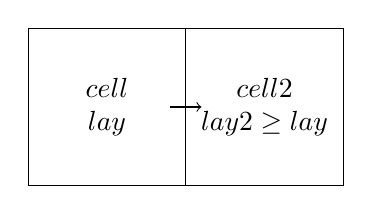
\begin{tikzpicture}[scale=2]
\draw(0,0)--(1,0)--(1,1)--(0,1)--cycle;
\node[align=center] at (0.5,0.5){$cell$\\$lay$};
\draw(1,0)--(2,0)--(2,1)--(1,1)--cycle;
\node[align=center] at (1.5,0.5){$cell2$\\$lay2\geq lay$};
\draw[->](0.9,0.5)--(1.1,0.5);
\end{tikzpicture}
}
\subcaptionbox{This is the case where the read is done in the same direction in negatif sign of the write.\label{code:fig:extrap:2}}{
\tikzset{external/export next=false}
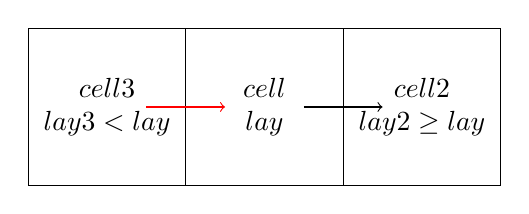
\begin{tikzpicture}[scale=2]
\draw(0,0)--(1,0)--(1,1)--(0,1)--cycle;
\draw(1,0)--(2,0)--(2,1)--(1,1)--cycle;
\draw(-1,0)--(0,0)--(0,1)--(-1,1)--cycle;
\draw[->](0.75,0.5)--(1.25,0.5);
\draw[->,red](-0.25,0.5)--(0.25,0.5);
\node[align=center] at (-0.5,0.5){$cell3$\\ $lay3<lay$};
\node[align=center] at (0.5,0.5){$cell$ \\$lay$};
\node[align=center] at (1.5,0.5){$cell2$ \\ $lay2\geq lay$};
\end{tikzpicture}
}
\subcaptionbox{This is the case where the read is done in the same direction in positif sign of the write.\label{code:fig:extrap:3}}
{
\tikzset{external/export next=false}
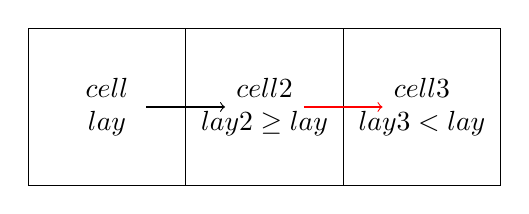
\begin{tikzpicture}[scale=2]
\draw(0,0)--(1,0)--(1,1)--(0,1)--cycle;
\draw(1,0)--(2,0)--(2,1)--(1,1)--cycle;
\draw(2,0)--(3,0)--(3,1)--(2,1)--cycle;
\draw[->](0.75,0.5)--(1.25,0.5);
\draw[->,red](1.75,0.5)--(2.25,0.5);
\node[align=center] at (2.5,0.5){$cell3$\\$lay3<lay$};
\node[align=center] at (1.5,0.5){$cell2$\\$lay2\geq lay$};
\node[align=center] at (0.5,0.5){$cell$\\$lay$};
\end{tikzpicture}
}
\subcaptionbox{This is the case where the read is done in a different direction of the write.\label{code:fig:extrap:4}}
{
\tikzset{external/export next=false}
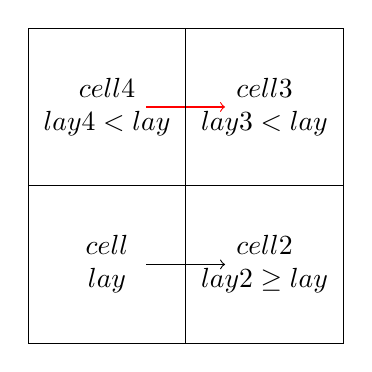
\begin{tikzpicture}[scale=2]
\draw(0,0)--(1,0)--(1,1)--(0,1)--cycle;
\draw(1,0)--(2,0)--(2,1)--(1,1)--cycle;
\draw[->](0.75,0.5)--(1.25,0.5);
\draw(0,1)--(1,1)--(1,2)--(0,2)--cycle;
\draw[->,red](0.75,1.5)--(1.25,1.5);
\draw(1,1)--(2,1)--(2,2)--(1,2)--cycle;
\node[align=center] at (0.5,1.5){$cell4$\\$lay4<lay$};
\node[align=center] at (1.5,1.5){$cell3$\\$lay3<lay$};
\node[align=center] at (0.5,0.5){$cell$\\$lay$};
\node[align=center] at (1.5,0.5){$cell2$\\$lay2\geq lay$};
\end{tikzpicture}
}
\caption{These are the cases used in algorithm \ref{code:AlgorithmsExtrapolateNan1}. These are cases where the speed component
is right the considered cell. In black is the speed component to set, in red is the speed component to read from.}
\end{center}
\end{figure}

\begin{figure}

\begin{center}
\subcaptionbox{The black speed component show a case considered when $lay$ has a given value.\label{code:fig:extrap:5}}
{
\tikzset{external/export next=false}
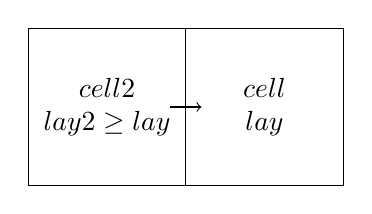
\begin{tikzpicture}[scale=2]
\draw(0,0)--(1,0)--(1,1)--(0,1)--cycle;
\node[align=center] at (0.5,0.5){$cell2$\\$lay2\geq lay$};
\draw(1,0)--(2,0)--(2,1)--(1,1)--cycle;
\node[align=center] at (1.5,0.5){$cell$\\$lay$};
\draw[->](0.9,0.5)--(1.1,0.5);
\end{tikzpicture}
}
\subcaptionbox{This is the case where the read is done in the same direction in positif sign of the write.\label{code:fig:extrap:6}}
{
\tikzset{external/export next=false}
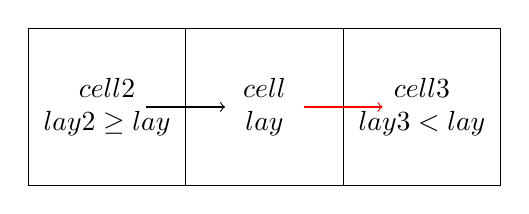
\begin{tikzpicture}[scale=2]
\draw(0,0)--(1,0)--(1,1)--(0,1)--cycle;
\draw(1,0)--(2,0)--(2,1)--(1,1)--cycle;
\draw(2,0)--(3,0)--(3,1)--(2,1)--cycle;
\draw[->](0.75,0.5)--(1.25,0.5);
\draw[->,red](1.75,0.5)--(2.25,0.5);
\node[align=center] at (2.5,0.5){$cell3$ \\ $lay3<lay$};
\node[align=center] at (1.5,0.5){$cell$\\$lay$};
\node[align=center] at (0.5,0.5){$cell2$ \\$lay2\geq lay$};
\end{tikzpicture}
}
\subcaptionbox{This is the case where the read is done in the same direction in negatif sign of the write.\label{code:fig:extrap:7}}
{
\tikzset{external/export next=false}
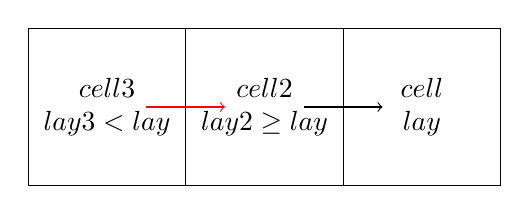
\begin{tikzpicture}[scale=2]
\draw(0,0)--(1,0)--(1,1)--(0,1)--cycle;
\draw(1,0)--(2,0)--(2,1)--(1,1)--cycle;
\draw(-1,0)--(0,0)--(0,1)--(-1,1)--cycle;
\draw[->](0.75,0.5)--(1.25,0.5);
\draw[->,red](-0.25,0.5)--(0.25,0.5);
\node[align=center] at (-0.5,0.5){$cell3$\\$lay3<lay$};
\node[align=center] at (0.5,0.5){$cell2$\\ $lay2\geq lay$};
\node[align=center] at (1.5,0.5){$cell$\\$lay$};
\end{tikzpicture}
}
\subcaptionbox{This is the case where the read is done in a different direction of the write.\label{code:fig:extrap:8}}
{
\tikzset{external/export next=false}
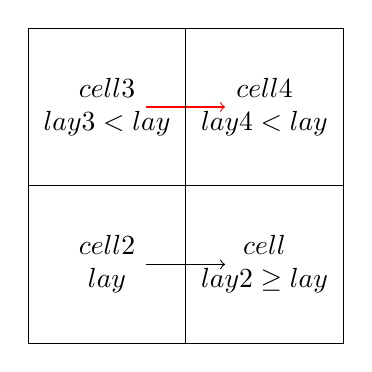
\begin{tikzpicture}[scale=2]
\draw(0,0)--(1,0)--(1,1)--(0,1)--cycle;
\draw(1,0)--(2,0)--(2,1)--(1,1)--cycle;
\draw[->](0.75,0.5)--(1.25,0.5);
\draw(0,1)--(1,1)--(1,2)--(0,2)--cycle;
\draw[->,red](0.75,1.5)--(1.25,1.5);
\draw(1,1)--(2,1)--(2,2)--(1,2)--cycle;
\node[align=center] at (0.5,1.5){$cell3$ \\ $lay3<lay$};
\node[align=center] at (1.5,1.5){$cell4$ \\ $lay4<lay$};
\node[align=center] at (0.5,0.5){$cell2$ \\ $lay$};
\node[align=center] at (1.5,0.5){$cell$\\ $lay2\geq lay$};
\end{tikzpicture}
}
\end{center}
\caption{These are the cases used in algorithm \ref{code:AlgorithmsExtrapolateNan2}. These are cases where the speed component
is left the considered cell. In black is the speed component to set, in red is the speed component to read from.}
\end{figure}

\begin{figure}

\begin{center}
\subcaptionbox{The black speed component show a case considered when $lay$ has a given value.\label{code:fig:extrap:9}}
{
\tikzset{external/export next=false}
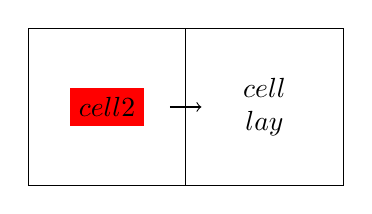
\begin{tikzpicture}[scale=2]
\draw(0,0)--(1,0)--(1,1)--(0,1)--cycle;
\node[align=center,fill=red] at (0.5,0.5){$cell2$};
\draw(1,0)--(2,0)--(2,1)--(1,1)--cycle;
\node[align=center] at (1.5,0.5){$cell$\\$lay$};
\draw[->](0.9,0.5)--(1.1,0.5);
\end{tikzpicture}
}
\subcaptionbox{This is the case where the read is done in the same direction in positif sign of the write.\label{code:fig:extrap:10}}
{
\tikzset{external/export next=false}
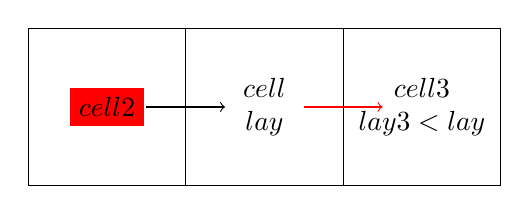
\begin{tikzpicture}[scale=2]
\draw(0,0)--(1,0)--(1,1)--(0,1)--cycle;
\draw(1,0)--(2,0)--(2,1)--(1,1)--cycle;
\draw(2,0)--(3,0)--(3,1)--(2,1)--cycle;
\draw[->](0.75,0.5)--(1.25,0.5);
\draw[->,red](1.75,0.5)--(2.25,0.5);
\node[align=center] at (2.5,0.5){$cell3$ \\ $lay3<lay$};
\node[align=center] at (1.5,0.5){$cell$\\$lay$};
\node[align=center,fill=red] at (0.5,0.5){$cell2$};
\end{tikzpicture}
}
\subcaptionbox{This is the case where the read is done in the same direction in negatif sign of the write.\label{code:fig:extrap:11}}
{
\tikzset{external/export next=false}
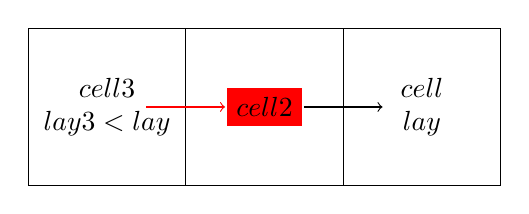
\begin{tikzpicture}[scale=2]
\draw(0,0)--(1,0)--(1,1)--(0,1)--cycle;
\draw(1,0)--(2,0)--(2,1)--(1,1)--cycle;
\draw(-1,0)--(0,0)--(0,1)--(-1,1)--cycle;
\draw[->](0.75,0.5)--(1.25,0.5);
\draw[->,red](-0.25,0.5)--(0.25,0.5);
\node[align=center] at (-0.5,0.5){$cell3$\\$lay3<lay$};
\node[align=center,fill=red] at (0.5,0.5){$cell2$};
\node[align=center] at (1.5,0.5){$cell$\\$lay$};
\end{tikzpicture}
}       
\subcaptionbox{This is the case where the read is done in a different direction of the write.\label{code:fig:extrap:12}}
{
\tikzset{external/export next=false}
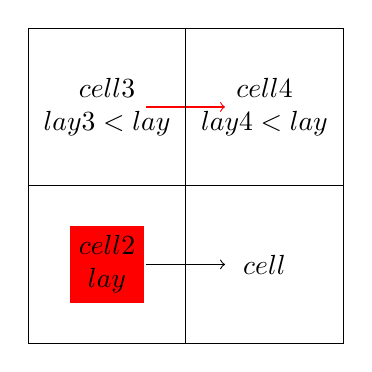
\begin{tikzpicture}[scale=2]
\draw(0,0)--(1,0)--(1,1)--(0,1)--cycle;
\draw(1,0)--(2,0)--(2,1)--(1,1)--cycle;
\draw[->](0.75,0.5)--(1.25,0.5);
\draw(0,1)--(1,1)--(1,2)--(0,2)--cycle;
\draw[->,red](0.75,1.5)--(1.25,1.5);
\draw(1,1)--(2,1)--(2,2)--(1,2)--cycle;
\node[align=center] at (0.5,1.5){$cell3$ \\ $lay3<lay$};
\node[align=center] at (1.5,1.5){$cell4$ \\ $lay4<lay$};
\node[align=center,fill=red] at (0.5,0.5){$cell2$ \\ $lay$};
\node[align=center] at (1.5,0.5){$cell$};
\end{tikzpicture}
}
\end{center}
\caption{These are the cases used in algorithm \ref{code:AlgorithmsExtrapolateNan3}. These are the cases where the speed component
is left the considered cell but where the left cell doesn't exist. In black is the speed component to set, in red is the speed component to read from. The cell marked in red doesn't exist, we cannot access left and below speed of them.}
\end{figure}
\subsection{Interpolation}

We will now show the pseudo code for interpolation for $N$ dimension with $N$-linear interpolation.
The principal difficulty is that on a staggered grid the position of known speed varie for all components.
The algorithm needed to do the translation is shown in algorithm \ref{code:GetSpeed}.
The interpolation is shown in algorithm \ref{code:GetSpeedImpl}.

\begin{algorithm}
\caption{Algorithm which calculate recursively the interpolation for scaled position in the square in range $[0,1]\times[0,1]$.}
\label{code:GetSpeedImpl}
\begin{algorithmic}[1]
\Function{GetSpeedImpl}{$posscal,i,cell,k$}\Comment{Get the interpolated speed in direction $k$ at position $posscal$ for cell $cell$.
$i$ is the recursif parameter it's first value should be 1.}
\State $cell2 \gets cell.\FuncCall{GetNeighbour}(i,1)$\Comment{We set $cell2$ to access speed in the other side in direction $i$.}
		\If{$i<dim$}\Comment{We are not in a terminal case, we do a linear interpolation in direction $i$ and recurse the linear interpolation in the rest
		of the dimension. The cell variable $cell2$ is used because it's ``origine'' of the second function call.}
			\State $ret \gets (1-posscal.\FuncCall{Get}(i))\cdot \FuncCall{GetSpeedImpl}(posscal,i+1,cell,k)+posscal.\FuncCall{Get}(i)\cdot \FuncCall{GetSpeedImpl}(posscal,i+1,cell2,k)$
			\State \Return $ret$
		\Else \Comment{We are in a terminal case. We acess the speed and do the linear interpolation.}
			\State $ret\gets (1-posscal.\FuncCall{Get}(i))*(cell.\FuncCall{SpeedGet}(k))+posscal.\FuncCall{Get}(i)*(cell2.\FuncCall{SpeedGet}(k))$
			\State \Return $ret$
		\EndIf
\EndFunction
\end{algorithmic}
\end{algorithm}

\begin{algorithm}
\caption{Algorithm which interpolate the speed at a given position.}
\label{code:GetSpeed}
\begin{algorithmic}[1]
\Function{GetSpeed}{$pos$}
		\For{$i=1 \To dim$}
			\State $posdelta.\FuncCall{Set}(i,\frac{pos.\FuncCall{Get}(i)}{h.\FuncCall{Get}(i)})$
			\Comment{Scale the position.}
			\State $key0.\FuncCall{Set}(i,round(pos_delta.GetRef(i)))$
			\Comment{We round to the nearest integer to find in which integer cell is the particle.}
			\State $posdelta.\FuncCall{Set}(i,posdelta.\FuncCall{Get}(i)-key0.\FuncCall{Get}(i))$
			\Comment{Because we have rounded to the nearest integer the value of $posdelta$ are in $[-0.5,0.5[$ 
			(the exact up or down rounding depend on the specification of the rounding function).}
		\EndFor
		\For{$k=1\To dim$}\Comment{For every speed component.}
			\State $posdelta.\FuncCall{Set}(k,posdelta.\FuncCall{Get}(k)+0.5)$\Comment{Because we are in a staggered grid the position is translated.
			The $0$ vector is at cell center. The range of $posdelta.\FuncCall{Get}(k)$ is in range $[0,1[$.}
			\For{$j=1 \To dim$}
				\If{$j\neq k$}\Comment{We loop on every speed component different than the used one.}
					\If{$posdelta.\FuncCall{Get}(j)<0$}\Comment{$posdelta.\FuncCall{Get}(j)$ is in range $[-0.5,0.5[$.}
						\State $key.\FuncCall{Set}(j,key0.\FuncCall{GetRef}(j)-1)$ \Comment{We go to the cell below because we have rounded to the cell above.}
						\State $posdelta2.\FuncCall{Set}(j,1+posdelta.\FuncCall{Get}(j))$ \Comment{We change the $posdelta2$ to the translation.
						$posdelta2.\FuncCall{Get}(j)$ is now in range $[0,1[$.}
					\Else
						\State $key.\FuncCall{Set}(j,key0.\FuncCall{Get}(j))$
						\State $posdelta2.\FuncCall{Set}(j,posdelta.\FuncCall{Get}(j))$
					\EndIf
				\Else
					\State $key.\FuncCall{Set}(j,key0.\FuncCall{Get}(j))$
					\State $posdelta2.\FuncCall{Set}(j,posdelta.\FuncCall{Get}(j))$
				\EndIf
			\EndFor
			\State $cell\gets Grid[key]$\Comment{We get the cell at the calculated $key$.}
			\State $ret.\FuncCall{Set}(k,\FuncCall{GetSpeedImpl}(pos_delta2,1,cell,k))$ \Comment{We call the interpolation routine and set the result in the return vector.}
			\State $posdelta.\FuncCall{Set}(k,posdelta.\FuncCall{Get}(k)-0.5)$
		\EndFor
		\State \Return $ret$
	\EndFunction
\end{algorithmic}
\end{algorithm}

\subsection{Integration}

For the non split case the acceleration is given by (\ref{topo:equ:onediff}).
We use to avoid to rewrite an extrapolation fonction a method $\FuncCall{SetSpeedToAcceleration}(bool)$
which toggles that the method to set the speed and get the speed act on acceleration instead.
This is shown in algorithm \ref{code:CalculateAcceleration2}

We now integrate with the Runge-Kutta method, the difference with respect to the case in section \ref{fixed:sec:rungekutta}
is that we now have particles. We need to do the same that we have done having a copy of all particle positions.
This is shown in algorithm \ref{code:RungeKutta2p1} and \ref{code:RungeKutta2p2}.

A complete iteration consists of Algorithm \ref{code:RungeKutta3}

\begin{algorithm}
\caption{Calculate the acceleration for the non split method equation (\ref{topo:equ:onediff}).}
\label{code:CalculateAcceleration2}
\begin{algorithmic}[1]
\Procedure{CalculateAcceleration2}{}
	\State $\FuncCall{InitializationRungeKutta}()$
	\State $\FuncCall{Do2dBoundaryExtrapolation}()$
	\State $\FuncCall{AlgorithmsExtrapolateNan}()$
	\State $\FuncCall{CalculateAcceleration}()$
	\State $\FuncCall{SetSpeedToAcceleration}(\True)$
	\State $\FuncCall{Do2dBoundaryExtrapolation}()$
	\State $\FuncCall{AlgorithmsExtrapolateNan}()$
	\State $\FuncCall{SetSpeedToAcceleration}(\False)$
\EndProcedure
        \end{algorithmic}
\end{algorithm}


\begin{algorithm}
\caption{Algorithm that integrate with the Runge Kutta method first part.}
\label{code:RungeKutta2p1}
\begin{algorithmic}[1]
\Procedure{RungeKutta}{}
\ForAll{$it\in Grid$}
            \State $it.\FuncCall{AccelerationSet}(0)$
            \Comment{We set the acceleration to $0$. So that we can after calculate the acceleration.}
\EndFor
	\State $\FuncCall{CalculateAcceleration}()$
	\Comment{This function will add the acceleration to the acceleration array.}
        \ForAll{$it \in Grid$}
            \State $it.\FuncCall{GetArray}(2).\FuncCall{SpeedSet}(it.\FuncCall{GetArray}(0).\FuncCall{SpeedGet}()+it.\FuncCall{AccelerationGet}()\cdot dt \cdot 0.5)$
            \Comment{Array $2$ is set to the speed for the next evaluation. We do not use array $0$ because we need it.}
            \State $it.\FuncCall{GetArray}(1).\FuncCall{SpeedSet}(it.\FuncCall{GetArray}(0).\FuncCall{SpeedGet}()+it.\FuncCall{AccelerationGet}()\cdot \frac{dt}{6})$
            \Comment{Array $1$ is set to the accumulation of the result.}
        \EndFor
                \ForAll{$it \in Particles$}
            \State $it.\FuncCall{GetList}(2).\FuncCall{PositionSet}(it.\FuncCall{GetList}(0).\FuncCall{PositionGet}()+it.\FuncCall{GetSpeed}(it.PositionGet())\cdot dt \cdot 0.5)$
            \Comment{List $2$ is set to the position for the next evaluation. We do not use list $0$ because we need it.}
            \State $it.\FuncCall{GetList}(1).\FuncCall{PositionSet}(it.\FuncCall{GetList}(0).\FuncCall{PositionGet}()+it.\FuncCall{GetSpeed}(it.PositionGet())\cdot \frac{dt}{6})$
            \Comment{List $1$ is set to the accumulation of the result.}
        \EndFor
        \ForAll{$it \in Grid$}
            \State $it.\FuncCall{AccelerationSet}(0)$
        \EndFor
        \State $\FuncCall{SetArraySpeed}(2)$
        \Comment{The speed for the next evaluation is in array $2$. We set array $2$ as default.}
        \State $\FuncCall{SetListPos}(2)$
        \Comment{The position of particle for the next evaluation is in list $2$. We set list $2$ as default.}
        \State $t\gets t+0.5\cdot dt$
        \State $\FuncCall{CalculateAcceleration}()$
        \ForAll{$it \in Grid$}
            \State $it.\FuncCall{GetArray}(2).\FuncCall{SpeedSet}(it.\FuncCall{GetArray}(0).\FuncCall{SpeedGet}()+it.\FuncCall{AccelerationGet}()\cdot \frac{dt}{2})$
            \Comment{Array $2$ is set to the speed for the next evaluation. We do not use array $0$ because we need it.}
            \State $it.\FuncCall{GetArray}(1).\FuncCall{SpeedSet}(it.\FuncCall{GetArray}(1).\FuncCall{SpeedGet}()+it.\FuncCall{AccelerationGet}()\cdot \frac{dt}{3})$
	    \Comment{Array $1$ is set to the accumulation of the result.}
       \EndFor
       \ForAll{$it \in Particles$}
            \State $it.\FuncCall{GetList}(2).\FuncCall{PositionSet}(it.\FuncCall{GetList}(0).\FuncCall{PositionGet}()+it.\FuncCall{GetSpeed}(it.PositionGet())\cdot \frac{dt}{2})$
            \Comment{List $2$ is set to the position for the next evaluation. We do not use list $0$ because we need it.}
            \State $it.\FuncCall{GeList}(1).\FuncCall{PositionSet}(it.\FuncCall{GetList}(1).\FuncCall{PositionGet}()+it.\FuncCall{GetSpeed}(it.PositionGet())\cdot \frac{dt}{3})$
	    \Comment{List $1$ is set to the accumulation of the result.}
       \EndFor
        \ForAll{$it\in Grid$}
            \State $it.\FuncCall{AccelerationSet}(0)$
        \EndFor
        \State $\FuncCall{CalculateAcceleration}()$
        \ForAll{$it \in Grid$}
            \State $it.\FuncCall{GetArray}(2).\FuncCall{SpeedSet}(it.\FuncCall{GetArray}(0).\FuncCall{SpeedGet}()+it.\FuncCall{AccelerationGet}()\cdot dt)$
            \State $it.\FuncCall{GetArray}(1).\FuncCall{SpeedSet}(it.\FuncCall{GetArray}(1).\FuncCall{SpeedGet}()+it.\FuncCall{AccelerationGet}()\cdot \frac{dt}{3})$
        \EndFor
         \ForAll{$it \in Particles$}
            \State $it.\FuncCall{GetList}(2).\FuncCall{PositionSet}(it.\FuncCall{GetList}(0).\FuncCall{PositionGet}()+it.\FuncCall{GetSpeed}(it.PositionGet())\cdot dt)$
            \State $it.\FuncCall{GetList}(1).\FuncCall{PositionSet}(it.\FuncCall{GetList}(1).\FuncCall{PositionGet}()+it.\FuncCall{GetSpeed}(it.PositionGet())\cdot \frac{dt}{3})$
        \EndFor
        \ForAll{$it \in Grid$}
            \State $it.\FuncCall{AccelerationSet}(0)$
        \EndFor
        \algstore{code:Rungekutta2:break:1}
             \end{algorithmic}
\end{algorithm}
\begin{algorithm}
\caption{Algorithm that integrate with the Runge Kutta method second part.}
\label{code:RungeKutta2p2}
\begin{algorithmic}[1]
\algrestore{code:Rungekutta2:break:1}
        \State $t\gets t+\frac{dt}{2}$
        \State $\FuncCall{CalculateAcceleration}()$
        \ForAll{$it\in Grid$}
            \State $it.\FuncCall{GetArray}(0).\FuncCall{SpeedSet}(it.\FuncCall{GetArray}(1).\FuncCall{SpeedGet}()+it.\FuncCall{AccelerationGet}()\cdot \frac{dt}{6})$
            \Comment{ Array $0$ now contain the new speed.}
         \EndFor
         \ForAll{$it\in Particles$}
            \State $it.\FuncCall{GetList}(0).\FuncCall{PositionSet}(it.\FuncCall{GetList}(1).\FuncCall{PositionGet}()+it.\FuncCall{GetSpeed}(it.PositionGet())\cdot \frac{dt}{6})$
            \Comment{ Array $0$ now contain the new speed.}
         \EndFor
        \State $\FuncCall{SetArraySpeed}(0)$
        \Comment{We set the default array again to $0$ to be ready for the next time step.}
        \State $\FuncCall{SetListPosition}(0)$
        \Comment{We set the default list again to $0$ to be ready for the next time step.}
        \EndProcedure
        \end{algorithmic}
\end{algorithm}

\begin{algorithm}
\caption{Algorithm one iteration.}
\label{code:RungeKutta3}
\begin{algorithmic}[1]
\Procedure{Iteration}{}
\State $\FuncCall{Initialisation}()$
\State $\FuncCall{RungeKutta}()$
\EndProcedure
        \end{algorithmic}
\end{algorithm}

\FloatBarrier
\section{Numerical experiments}

\subsection{One particle fall}
\label{top:exp:one}
We have discussed this case qualitatively, we will now simulate it numerically.

We take as initial condition a single particle with 0 speed everywhere without viscosity falling from gravity.

The analytical solution is for the continuous problem given by:
\begin{align}
v&=-gt\\
x&=x_0-\frac{1}{2}gt^2
\end{align}

If we add viscosity the same is true.

\subsubsection{Result}

We see in figure \ref{topo:singl_part:fig1} and \ref{topo:singl_part:fig2} that the non split method coincides with the analytical solution for the
integration method Runge-Kutta of order 4. The reason is that the analytical solution is a polynomial of order 2.

In contrast, because of the splitting, a splitting method will incorrectly approximate the result, because it is of order 1 at general.

When we have big time steps like $\alpha=2$ the non split method behaves better. But it is important to recall the results on fixed grid,
that having a too big time step make diverge.

\begin{figure}
\includegraphics{topology/single_part/tab2.pdf}
\caption{Comparison between splitting and not splitting for a single particle problem. 
The integration method is Runge-Kutta of order 4 for the two case.
We see that the non split method is a very good approximation to the analytical solution.
Instead the split method  and is different than the analytical solution.
For the two methods, we have used $\Delta x=0.01$. The time step limiter was a maximal time step $dt_{max}=0.01$.
}
\label{topo:singl_part:fig1}
\end{figure}

\begin{figure}
\includegraphics{topology/single_part/tab.pdf}
\caption{Comparison between splitting and not splitting for a single particle problem. 
The integration method is Runge-Kutta of order 4 for the two case.
We see that the non split method is a very good approximation to the analytical solution.
Instead the split method  and is different than the analytical solution.
For the two methods, we have used $\Delta x=0.01$. The time step limiter was a maximal time step $dt_{max}=0.01$.
We do not know why we have small jump in precision for split method.}
\label{topo:singl_part:fig2}
\end{figure}

\subsection{Lateral jet}

We consider a continuous source of speed in the $x$ direction, with gravity in the $y$ direction.
The analytical solution can be found without consideration of the boundary condition.

A single particle with initial $x$ speed $v_{0}$ which go from $y$ position $y_0$ and with initial time $t_0$.

The speed is:
\begin{align}
	v_{x}&=v_{0}\\
	v_{y}&=-\frac{g}{2}(t-t_0)^2
\end{align}

The position of the particle is then:
\begin{align}
	x&=v_{0}(t-t_0)\\
	y&=y_0-\frac{g}{2}(t-t_0)^2
\end{align}

We will now try to define the speed in a particle manner.
The time is given by:
\begin{equation}
	t-t_{0}=\frac{x}{v_{0}}
\end{equation}

The speed is then given by:
\begin{align}
	v_{x}&=v_{0}\\
	v_{y}&=-\frac{g}{2}\frac{x^2}{v_{0}}
\end{align}
This is divergence free.
So we are a solution of the Navier-Stokes equation.

But we does not respect the boundary condition.

We cannot know apriori if the numerical solution with correct boundary condition will respect this solution.
But we can expect that a perturbation at boundary that will respect the boundary condition,
will rest in the boundary and not enter in the fluid.
This approximation is called Boundary Layer.


\subsubsection{Results}


For the numerical method, we have added a small perturbation in the initial $x$ speed.

We see in figure \ref{topo:extrap:lateral:8_1}, \ref{topo:extrap:lateral:9_1} and \ref{topo:extrap:lateral:10_1} that lateral
speed are smoothed by the viscosity and is quasi constant which is the analytical solution.

The boundary of the analytical solution is near to the numerical solution.
Only the end of the fluid does not follow the analytical solution.
This indicates that boundary layers are  correctly approximated.
\begin{figure}
	\includegraphics{topology/lateral_jet/plot_8__1_186.pdf}
	\caption{Non split result with Runge-Kutta rk4 with $\nu=1.307e-6$, $\alpha=0.5$.
	This is the $x$ speed.
	The green line is the analytical solution boundary for the result without boundary condition.
	The blue line is the calculate boundary.
	We see that except at the end, the two coincide.
	At interior the speed take the analytical value which is constant and has a little jump in the boundary.
	The perturbation at initial condition are smirred by the viscosity.}
	\label{topo:extrap:lateral:8_1}
\end{figure}

\begin{figure}
	\includegraphics{topology/lateral_jet/plot_8__2_186.pdf}
	\caption{Non split result with Runge-Kutta rk4 with $\nu=1.307e-6$, $\alpha=0.5$.
	This is the $y$ speed.
	The green line is the analytical solution boundary for the result without boundary condition.
	The blue line is the calculate boundary.
	We see that except at the end, the two coincide.
	The $y$ speed is proportional to the $x^2$ position, which coincide with the analytical result.
	The perturbation at initial condition are smirred by the viscosity.}
	\label{topo:extrap:lateral:8_2}
\end{figure}

\begin{figure}
	\includegraphics{topology/lateral_jet/plot_new__1.pdf}
		\caption{Split result with Runge-Kutta rk4 with $\nu=1.307e-6$, $\alpha=0.5$.
	This is the $x$ speed.
	The green line is the analytical solution boundary for the result without boundary condition.
	The blue line is the calculate boundary.
	We see that except at the end, the two coincide.
	At interior the speed take the analytical value which is constant and has a little jump in the boundary.
	The perturbation at initial condition are smirred by the viscosity.}
	\label{topo:extrap:lateral:9_1}
\end{figure}

\begin{figure}
	\includegraphics{topology/lateral_jet/plot_new__2.pdf}
		\caption{Split result with Runge-Kutta rk4 with $\nu=1.307e-6$, $\alpha=0.5$.
	This is the $y$ speed.
	The green line is the analytical solution boundary for the result without boundary condition.
	The blue line is the calculate boundary.
	We see that except at the end, the two coincide.
	The $y$ speed is proportional to the $x^2$ position, which coincide with the analytical result.
	The perturbation at initial condition are smirred by the viscosity.}
	\label{topo:extrap:lateral:9_2}
\end{figure}


\begin{figure}
	\includegraphics{topology/lateral_jet/plot_10__1_293.pdf}
			\caption{Split result with Euler with $\nu=1.307e-6$, $\alpha=0.5$.
	This is the $x$ speed.
	The green line is the analytical solution boundary for the result without boundary condition.
	The blue line is the calculate boundary.
	We see that except at the end, the two coincide.
	At interior the speed take the analytical value which is constant and has a little jump in the boundary.
	The perturbation at initial condition are smirred by the viscosity.}
	\label{topo:extrap:lateral:10_1}
\end{figure}

\begin{figure}
	\includegraphics{topology/lateral_jet/plot_10__2_293.pdf}
			\caption{Split result with Euler with $\nu=1.307e-6$, $\alpha=0.5$.
	This is the $y$ speed.
	The green line is the analytical solution boundary for the result without boundary condition.
	The blue line is the calculate boundary.
	We see that except at the end, the two coincide.
	The $y$ speed is proportional to the $x^2$ position, which coincide with the analytical result.
	The perturbation at initial condition are smirred by the viscosity.}
	\label{topo:extrap:lateral:10_2}
\end{figure}


\subsection{Jet}

We now try to simulate the same problem as the lateral jet but in the same direction of gravity.
We have no analytical solution in this case because the trivial particle solution is no more divergence free.
Pressure is needed to push the fluid up.

We have done two final numerical runs of this problem.
All numerical run were done with 50 cells at the basis. With a spacing of $\unit{0.0002}{\meter}$.
The viscosity is $\nu=\unit{1.307\cdot 10^{-6}}{\meter \squared \per\second}$ which is the viscosity of water.
We use $\alpha=0.5$. We use the non split rk4 integration method.
Particles which go below the 0 altitude are supressed.

The two runs took a day to complete. 3 dimensional runs were not possible for reasons of time and
computing power.

This is shown in figure \ref{top:jet:G}, \ref{top:jet:Gx}, \ref{top:jet:Gy}, \ref{top:jet:P}, \ref{top:jet:Px} and
\ref{top:jet:Py}.

The most expensive operation is to calculate the projection operator for every iteration.

We see three phases in the computed result:
\begin{enumerate}
 \item Vertical motion without deformation. Gravity had not the time to act a lot on the speed.
 \item The top particles want to push the below particles because of gravity.
 But because of incompressibility the below region becomes larger. This generates
 a lateral speed.
 \item We touch the supression particles limit and have now a stationary state.
\end{enumerate}

We think that the reason why the jet lateral distance is so big is because we are in a 2d problem where
we have less spatial liberty. The pressure exerted by the gravity can in 2d escape only in one dimension
and not two.

\begin{figure}
\begin{center}
\subcaptionbox{\label{top:jet:G:1}}
{
\includegraphics[width=0.4\textwidth]{topology/JetGrand/topo0001.jpg}
}
\subcaptionbox{\label{top:jet:G:2}}
{
\includegraphics[width=0.4\textwidth]{topology/JetGrand/topo0002.jpg}
}
\subcaptionbox{\label{top:jet:G:3}}
{
\includegraphics[width=0.4\textwidth]{topology/JetGrand/topo0003.jpg}
}
\subcaptionbox{\label{top:jet:G:4}}
{
\includegraphics[width=0.4\textwidth]{topology/JetGrand/topo0004.jpg}
}
\subcaptionbox{\label{top:jet:G:5}}
{
\includegraphics[width=0.4\textwidth]{topology/JetGrand/topo0005.jpg}
}
\subcaptionbox{\label{top:jet:G:6}}
{
\includegraphics[width=0.4\textwidth]{topology/JetGrand/topo0006.jpg}
}
\end{center}
\caption{Jet simulation with an initial speed $\unit{2}{\meter \per \second}$.
The red region is the region with fluid. The black surface are in fact the particles.}
\label{top:jet:G}
\end{figure}

\begin{figure}
\begin{center}
\subcaptionbox{\label{top:jet:Gx:1}}
{
\includegraphics[width=0.4\textwidth]{topology/JetGrand/speedx0001.jpg}
}
\subcaptionbox{\label{top:jet:Gx:2}}
{
\includegraphics[width=0.4\textwidth]{topology/JetGrand/speedx0002.jpg}
}
\subcaptionbox{\label{top:jet:Gx:3}}
{
\includegraphics[width=0.4\textwidth]{topology/JetGrand/speedx0003.jpg}
}
\subcaptionbox{\label{top:jet:Gx:4}}
{
\includegraphics[width=0.4\textwidth]{topology/JetGrand/speedx0004.jpg}
}
\subcaptionbox{\label{top:jet:Gx:5}}
{
\includegraphics[width=0.4\textwidth]{topology/JetGrand/speedx0005.jpg}
}
\subcaptionbox{\label{top:jet:Gx:6}}
{
\includegraphics[width=0.4\textwidth]{topology/JetGrand/speedx0006.jpg}
}
\end{center}
\caption{Jet simulation with an initial speed $\unit{2}{\meter \per \second}$.
This is the representation of speed in the $x$ direction.}
\label{top:jet:Gx}
\end{figure}

\begin{figure}
\begin{center}
\subcaptionbox{\label{top:jet:Gy:1}}
{
\includegraphics[width=0.4\textwidth]{topology/JetGrand/speedy0001.jpg}
}
\subcaptionbox{\label{top:jet:Gy:2}}
{
\includegraphics[width=0.4\textwidth]{topology/JetGrand/speedy0002.jpg}
}
\subcaptionbox{\label{top:jet:Gy:3}}
{
\includegraphics[width=0.4\textwidth]{topology/JetGrand/speedy0003.jpg}
}
\subcaptionbox{\label{top:jet:Gy:4}}
{
\includegraphics[width=0.4\textwidth]{topology/JetGrand/speedy0004.jpg}
}
\subcaptionbox{\label{top:jet:Gy:5}}
{
\includegraphics[width=0.4\textwidth]{topology/JetGrand/speedy0005.jpg}
}
\subcaptionbox{\label{top:jet:Gy:6}}
{
\includegraphics[width=0.4\textwidth]{topology/JetGrand/speedy0006.jpg}
}
\end{center}
\caption{Jet simulation with an initial speed $\unit{2}{\meter \per \second}$.
This is the representation of speed in the $y$ direction.}
\label{top:jet:Gy}
\end{figure}

\begin{figure}
\begin{center}
\subcaptionbox{\label{top:jet:P:1}}
{
\includegraphics[width=0.4\textwidth]{topology/JetPetit/topo0000.jpg}
}
\subcaptionbox{\label{top:jet:P:2}}
{
\includegraphics[width=0.4\textwidth]{topology/JetPetit/topo0001.jpg}
}
\subcaptionbox{\label{top:jet:P:3}}
{
\includegraphics[width=0.4\textwidth]{topology/JetPetit/topo0002.jpg}
}
\subcaptionbox{\label{top:jet:P:4}}
{
\includegraphics[width=0.4\textwidth]{topology/JetPetit/topo0003.jpg}
}
\subcaptionbox{\label{top:jet:P:5}}
{
\includegraphics[width=0.4\textwidth]{topology/JetPetit/topo0004.jpg}
}
\subcaptionbox{\label{top:jet:P:6}}
{
\includegraphics[width=0.4\textwidth]{topology/JetPetit/topo0005.jpg}
}
\end{center}
\caption{Jet simulation with an initial speed $\unit{1}{\meter \per \second}$.
The black surface are in fact the particles.}
\label{top:jet:P}
\end{figure}

\begin{figure}
\begin{center}
\subcaptionbox{\label{top:jet:Px:1}}
{
\includegraphics[width=0.4\textwidth]{topology/JetPetit/speedx0000.jpg}
}
\subcaptionbox{\label{top:jet:Px:2}}
{
\includegraphics[width=0.4\textwidth]{topology/JetPetit/speedx0001.jpg}
}
\subcaptionbox{\label{top:jet:Px:3}}
{
\includegraphics[width=0.4\textwidth]{topology/JetPetit/speedx0002.jpg}
}
\subcaptionbox{\label{top:jet:Px:4}}
{
\includegraphics[width=0.4\textwidth]{topology/JetPetit/speedx0003.jpg}
}
\subcaptionbox{\label{top:jet:Px:5}}
{
\includegraphics[width=0.4\textwidth]{topology/JetPetit/speedx0004.jpg}
}
\subcaptionbox{\label{top:jet:Px:6}}
{
\includegraphics[width=0.4\textwidth]{topology/JetPetit/speedx0005.jpg}
}
\end{center}
\caption{Jet simulation with an initial speed $\unit{1}{\meter \per \second}$.
This is the representation of speed in the $x$ direction.}
\label{top:jet:Px}
\end{figure}

\begin{figure}
\begin{center}
\subcaptionbox{\label{top:jet:Py:1}}
{
\includegraphics[width=0.4\textwidth]{topology/JetPetit/speedy0000.jpg}
}
\subcaptionbox{\label{top:jet:Py:2}}
{
\includegraphics[width=0.4\textwidth]{topology/JetPetit/speedy0001.jpg}
}
\subcaptionbox{\label{top:jet:Py:3}}
{
\includegraphics[width=0.4\textwidth]{topology/JetPetit/speedy0002.jpg}
}
\subcaptionbox{\label{top:jet:Py:4}}
{
\includegraphics[width=0.4\textwidth]{topology/JetPetit/speedy0003.jpg}
}
\subcaptionbox{\label{top:jet:Py:5}}
{
\includegraphics[width=0.4\textwidth]{topology/JetPetit/speedy0004.jpg}
}
\subcaptionbox{\label{top:jet:Py:6}}
{
\includegraphics[width=0.4\textwidth]{topology/JetPetit/speedy0005.jpg}
}
\end{center}
\caption{Jet simulation with an initial speed $\unit{1}{\meter \per \second}$.
This is the representation of speed in the $y$ direction.}
\label{top:jet:Py}
\end{figure}
\chapter{Conclusion}

In conclusion we were able to have a ``simple'' scheme to solve free surface incompressible 
Navier-Stokes equations.
For this we have used the following elements:
\begin{itemize}
 \item A spatial discretization on a staggered grid and the definition of a discretized differential operator on it.
 \item The reduction of the original problem to an ODE with a projected function.
 This needs to solve a linear system at every time step.
 \item A topological marker particle and interpolation method on the marker.
 \item An extrapolation operator that needs to ensure boundary conditions.
\end{itemize}

We were not able to launch 3d runs and are aware of the high numerical cost of direct Navier-Stokes
methods for small viscosity problems, but judged that it was the better method to begin with.

\section{Possible improvement}

The following theoretical improvements are possible:
\begin{itemize}
 \item Use higher order spatial discretization.
 \item Use other topological markers instead of particles like level sets or boundary surface representations.
 \item Have better discretization at the free surface boundary.
 \item Have a variant of the Runge-Kutta method that is correct if we have a Dirac delta in the function 
 or use smooth topological change.
\end{itemize}

The following code improvements are possible:
\begin{itemize}
 \item Have a linear solver which can use the fact that topology does not change much between iterations
 to be faster on average.
 \item Make the code run in parallel on cpus and gpus.
\end{itemize}

\section{Software used}

The code was written primary in \textbf{C++11}.
The final version uses the following libraries:
\begin{itemize}
 \item Umfpack as linear solver.
 \item VTK for output in the vtk format used in the visualization software Paraview.
\end{itemize}

Previous version used:
\begin{itemize}
 \item Boost library for python binding and externalization.
 \item Pyamg in python for multigrid.
 \item VianaCl for multigrid.
 \item Lusol in fortran for sparse Lu updating.
 \item Spooles as linear solver.
 \item \ldots
\end{itemize}

For postprocessing and generate this document the following software were used:
\begin{itemize}
 \item Lua\LaTeX \ as \LaTeX \ program with some lua script to generate picture.
 \item Pgfplots and tikz for picture and graphics.
 \item Matplotlib in python to generate picture and graphics.
 \item Paraview to visualize the data.
\end{itemize}

For debuging of the \textbf{C++11} code in addition to GDB, Valgrind was used to track memory
related error and memory leak.

\section{Thanks}

I am very thankfull to:
\begin{description}
 \item[Prof. Martin Gander:] for the supervising of the work and all my numerical analysis knowledge.
 \item[Dr. Félix Kwok:] for the supervising of the work and contact in practical numerical analysis.
 \item[Prof. Peter Wittwer:] for the Mathematics and Physics courses in my Physics studies.
 \item[My family: Reto, Norma, Roland, Tamara:] for supporting me and all the fun together.
 And for proof reading.
\end{description}


\bibliographystyle{plain}
\nocite{*}
\bibliography{main}
\end{document}